\documentclass[12pt,a4paper,BCOR=.7cm,headsepline,bibliography=totoc]{report}

\title{تحقیق در ویرایش ژنوم به کمک تناوب‌هایِ کوتاهِ پالیندرومِ فاصله‌دارِ منظمِ خوشه‌ای}

\usepackage{PersianTemplate}

\newcommand{\specialcell}[2][c]{%
  \begin{tabular}[#1]{@{}c@{}}#2\end{tabular}}

\makeindex

\logo{pictures/sharif-logo.png}
\university{دانشگاه صنعتی شریف }
\department{دانشکده علوم ریاضی}
\thesis{ پایان نامه کارشناسی‌ارشد}
\subject{‌ریاضی کاربردی}

\author{محمد رستمی }
\supervisor{دکتر محسن شریفی تبار}
\secsupervisor{دکتر حمیدرضا ربیعی}%در صورت نیاز
\advisor{دکتر محمدحسین رهبان}%در صورت نیاز
\date{\today}

\begin{document}
\makethesistitle
\signture{1}{2}{3}{4}
\thank{
با تشکر از دکتر ربیعی، دکتر رهبان، استاد راهنمای عزیزم دکتر شریفی‌تبار، امین قریاضی و حامد دشتی برای کمک‌های مداومشان،
}
\begin{abstract}
تناوب‌هایِ کوتاهِ پالیندرومِ فاصله‌دارِ منظمِ خوشه‌ای یا به طور خلاصه ، \lr{CRISPR} (کریسپر) یکی از روش‌های نسبتا نوین است که متخصصان ژنتیک و محققان پزشکی را قادر می سازد تا با حذف بخشهایی از ژنوم ،
افزودن یا تغییر بخش هایی از آن در \lr{dna} (دی‌ان‌ای) تغییر ایجاد کنند. این فناوری نوعی سیستم ایمنی تطابق‌پذیر در باکتری‌ها است که با کمک آن می‌توان بسیاری از بیماری‌ها مانند نابینوایی و ناشنوایی و حتی سرطان را درمان کرد. یکی از مشکلات بزرگ در استفاده موفق کریسپر، دقیق پیش‌بینی کردن تاثیر \lr{Guide RNA} (راهنمای آر‌ان‌ای) روی هدف و حساسیت خارج از هدف است. در حالی که برخی از روش ها این طرح ها را طبقه بندی می کنند ، بیشتر
الگوریتم ها بر روی داده های جداگانه با ژن ها و سلول های مختلف هستند. عدم تعمیم این روش ها
مانع استفاده از این راهنما در آزمایشات بالینی می شود ، زیرا برای هر درمان، این فرایند باید دقیقا برای همان سلول درست شده باشد و عموما داده کافی برای طراحی الگوریتم در آن سلول در دسترس نیست. ما سعی می‌کنیم مشکل تعمیم‌پذیری را حل کنیم و مدل‌ای ارائه دهیم که هم به‌صورت عمومی و هدفمند دقت خوبی داشته باشد تا که محققان در بهینه سازی طراح راهنمای آران‌ای با حساسیت مناسب کمک کند.
\end{abstract}
\pagestyle{plain}\pagenumbering{tartibi}

%دستورات بالا، قبل از شروع لیست مراجع و شکل و جدول و ... قرار می‌گیرد
\tableofcontents{} \listoffigures{}
\chapter{مقدمات}
\pagestyle{fancy} \pagenumbering{arabic}
 قبل از این که با کریسپر آشنا شویم، خوب است کمی راجع به تاریخچه ویرایش ژن‌ها صحبت کنیم. انسان‌ها سال‌هاست که مشغول به ویرایش و مهندسی ژن هستند، با استفاده از پرورش انتخابی\LTRfootnote{\lr{Selective Breeding}}.
	اصلاحات نژادی متعددی در گیاهان و حیوانات مخصوصا گونه‌های کلیدی مانند گندم، برنج و سگ‌ها ایجاد شده است. انسان‌ها در این کار شدیدا ماهر شدن به‌طوری که در صده گذشته، تعداد دانه‌های هر شاخه گندم چندین برابر و ارتفاع آنها کوتاه‌تر شده تا در معرض خطر کمتری باشند و حدود ۸۰ نژاد جدید سگ به وجود آمده است. البته با وجود پیشرفت‌های متعدد انسان‌ها تا کشف دی‌ان‌ای دقیقا ساز و کار آن را نمی دانستند. 
	
\section{RNA}
\begin{wrapfigure}{l}{6.75cm}
\centering
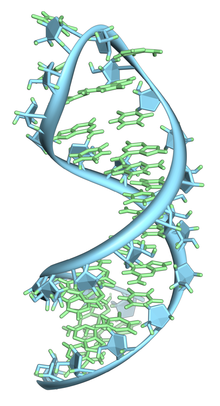
\includegraphics[width=2cm, height=4cm]{pictures/Pre-mRNA-1ysv-tubes.png}
\caption{
یک حلقه از pre-mRNA. نوکلئوبازها (سبز) و ستون فقرات ریبوز فسفات (آبی) مشخص شده اند. این یک رشته منفرد از RNA است که بر روی خود تا می شود.
}\label{wrap-fig:1}
\end{wrapfigure}
اسید ریبونوکلئیک\LTRfootnote{\lr{RiboNucleic Acid}} یا RNA
 یک مولکول پلیمری است که در نقش‌های بیولوژیکی مختلف مانند کدگذاری، رمزگشایی، تنظیم و بیان ژن‌ها ضروری است. RNA به صورت یک رشته منفرد از نوکلئوتیدها (بازهای نیتروژنی گوانین، اوراسیل، آدنین و سیتوزین که با حروف G، U، A و C مشخص می شوند) است که برخودش تا می خورد، بر خلاف دی‌ان‌ای که با یک رشته دیگر جفت شده است.
 
نوعی از RNA اطلاعات را از DNA به سیتوپلاسم حمل می‌کند؛ به این نوع RNA که اطلاعات را از DNA به ریبوزوم‌ها حمل می‌کند، RNA پیک یا پیامبر(mRNA) می‌گویند. نوعی دیگر از ،RNA
RNA
 حامل (tRNA) است که اسیدهای آمینه را به ریبوزوم منتقل می‌کند، تا ریبوزوم، اسیدهای آمینه را بر اساس اطلاعات موجود در mRNA کنار یکدیگر ردیف کند. نوع دیگر، RNA ریبوزومی (rRNA) است که در ساختار ریبوزوم‌ها شرکت دارد؛ این موضوع به این معناست که ریبوزوم (رناتن) ها متشکل از پروتئین ها و RNA های ریبوزومی هستند.
\section{دی‌ان‌ای}

دئوکسی ریبو نوکلئیک اسید\LTRfootnote{\lr{Deoxyribonucleic acid}} به اختصار دی‌اِن‌اِی یک مولکول متشکل از دو زنجیره پلی نوکلئوتیدی است که به دور یکدیگر می‌پیچند تا دستورالعمل‌های ژنتیکی برای کارکرد و توسعهٔ زیستی جانداران و ویروس‌ها مورد استفاده قرار می‌گیرد. نقش اصلی مولکول دی‌ان‌ای ذخیره‌سازی طولانی مدت اطلاعات ژنتیکی و دستوری است. لیپید‌ها، پروتئین‌ها، کربوهیدرات های پیچیده (پلی ساکاریدها) و اسیدهای نوکلئیک سه درشت‌مولکول‌های اصلی و ضروری برای همه اشکال شناخته شده حیات هستند.

دو رشته DNA به عنوان پلی نوکلئوتید شناخته می شوند زیرا از واحدهای مونومر یا تکپار ساده‌تری به نام نوکلئوتید تشکیل شده اند. هر نوکلئوتید از یکی از چهار نوکلئوباز حاوی نیتروژن (سیتوزین C، گوانین G، آدنین A یا تیمین T)،  کربوهیدرات پنج‌کربنه به نام دئوکسی ریبوز و یک گروه فسفات تشکیل شده است. نوکلئوتیدها در یک زنجیره توسط پیوندهای کووالانسی (معروف به پیوند فسفو دی استر) بین قند یک نوکلئوتید و فسفات نوکلئوتید بعدی به یکدیگر متصل می‌شوند و در نتیجه یک ستون فقرات قند-فسفات متناوب ایجاد می شود.
\begin{wrapfigure}{l}{6.5cm}
\centering
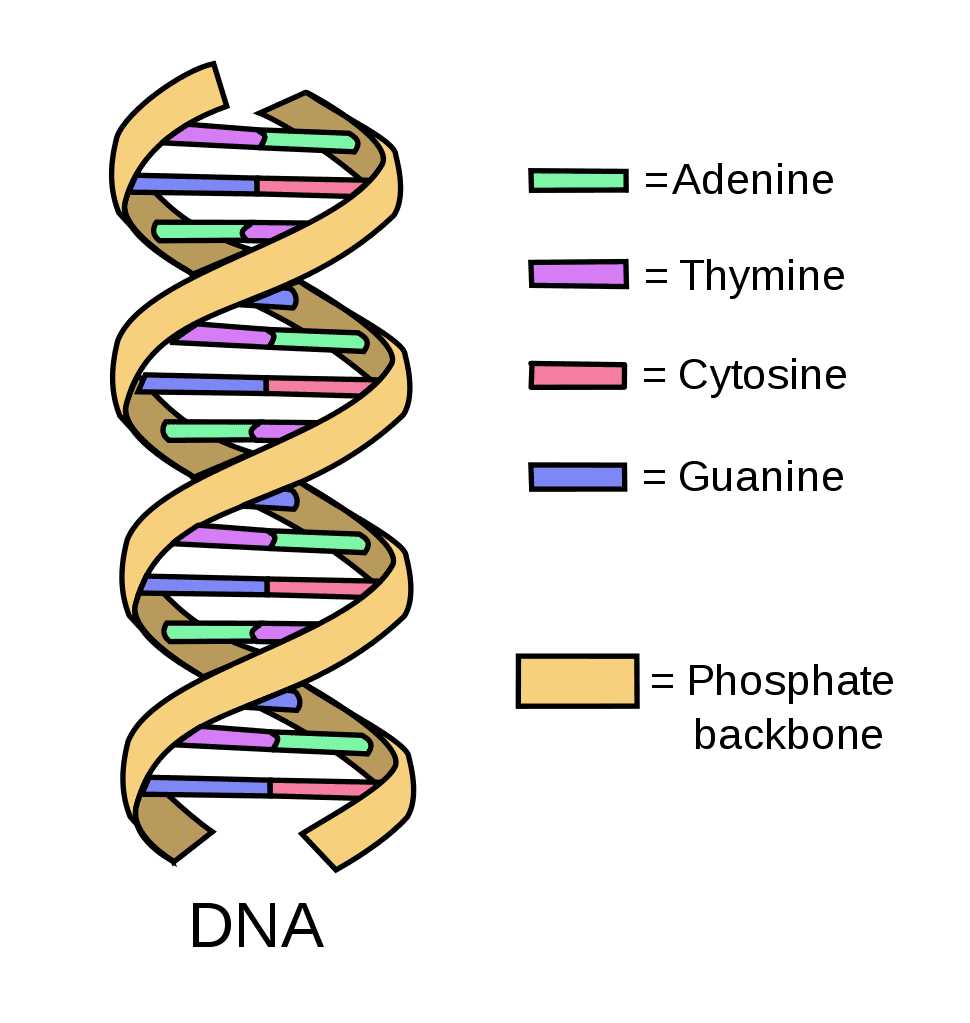
\includegraphics[width=4cm, height=5cm]{pictures/DNApng.png}
\caption{
شکل دو بعدی DNA
}\label{wrap-fig:2}
\end{wrapfigure}
 بازهای نیتروژنی دو رشته پلی نوکلئوتیدی جداگانه، طبق قوانین جفت شدن باز‌ها 
\lr{)}A با T و C با G\lr{(}
، با پیوندهای هیدروژنی به یکدیگر متصل می شوند تا DNA دو رشته‌ای بسازند. این دو رشته مکمل، ناهمسو و محلول (در آب) هستند (دی‌ان‌ای حلقوی قطبیت ندارد اما هر رشته از دی‌ان‌ای خطی دارای قطبیت است). بازهای نیتروژنی مکمل به دو گروه پیریمیدین‌ها و پورین‌ها تقسیم می شوند. در DNA، پیریمیدین ها تیمین و سیتوزین هستند. پورین‌ها آدنین و گوانین هستند.


هر دو رشته DNA اطلاعات بیولوژیکی یکسانی را ذخیره می‌کنند. این اطلاعات زمانی که دو رشته از هم جدا می‌شوند، تکرار می شود. بخش بزرگی از DNA (بیش از 98٪ برای انسان) بی‌کد\LTRfootnote{\lr{non-coding}}
 است، به این معنی که این بخش‌ها توالی‌های پروتئین را کد نمی‌کنند. دو رشته DNA در جهت مخالف یکدیگر قرار دارند و بنابراین باز مکمل ابتدای یک رشته آخر رشته دیگر هستند. در آیین نامگذاری ترکیبهای شیمیایی، اتمهای کربن در حلقهٔ شکری نوکلئوتید شماره‌گذاری شده‌اند. هر رشتهٔ دی‌ان‌ای یا آران‌ای دارای یک پایانهٔ '۵ که معمولا شامل یک گروه فسفاتی است و یک پایانهٔ '۳ که معمولاً از جانشین ریبوز اصلاح نشده -OH است. به هر قند یکی از چهار نوع نوکلئوباز (یا باز) متصل است. توالی این چهار هسته در امتداد ستون فقرات است که اطلاعات ژنتیکی را رمزگذاری می کند. رشته‌های RNA با استفاده از رشته‌های DNA به‌عنوان یک الگو در فرآیندی به نام رونویسی ایجاد می‌شوند که در آن بازهای DNA با بازهای مربوطه خود مبادله می‌شوند، به جز در مورد تیمین (T)، که RNA جایگزین اوراسیل (U) می‌شود. تحت کد ژنتیکی، این رشته‌های RNA توالی اسیدهای آمینه درون پروتئین‌ها را در فرآیندی به نام ترجمه مشخص می‌کنند.
\subsection{تفاوت‌های دی‌ان‌ای و آران‌ای}

تفاوت‌ها:
\begin{itemize}
\item DNA در ذخیره و RNA در انتقال اطلاعات وراثتی و در ساختار ریبوزوم نقش دارد.
\item مولکول DNA دو رشته‌ای در هم تنیده اما مولکول RNA تک‌رشته‌ای است.
\item 
در DNA باز آلی یوراسیل و در RNA باز آلی تیمین شرکت ندارد (U در DNA و T در RNA).
\item
قند پنج‌کربنه موجود در DNA را دئوکسی ریبوز و در RNA قند ریبوز نامیده می شود. تفاوت بین قندها وجود گروه هیدروکسیل بر روی کربن '۲ ریبوز و عدم وجود آن در کربن '۲ دئوکسی ریبوز است.
\item DNA برعکس RNA از هستهٔ سلول خارج نمی‌شود.
\item RNA بدون ژن می‌باشد.

\end{itemize}
{\begin{wrapfigure}{l}{10cm}
\centering
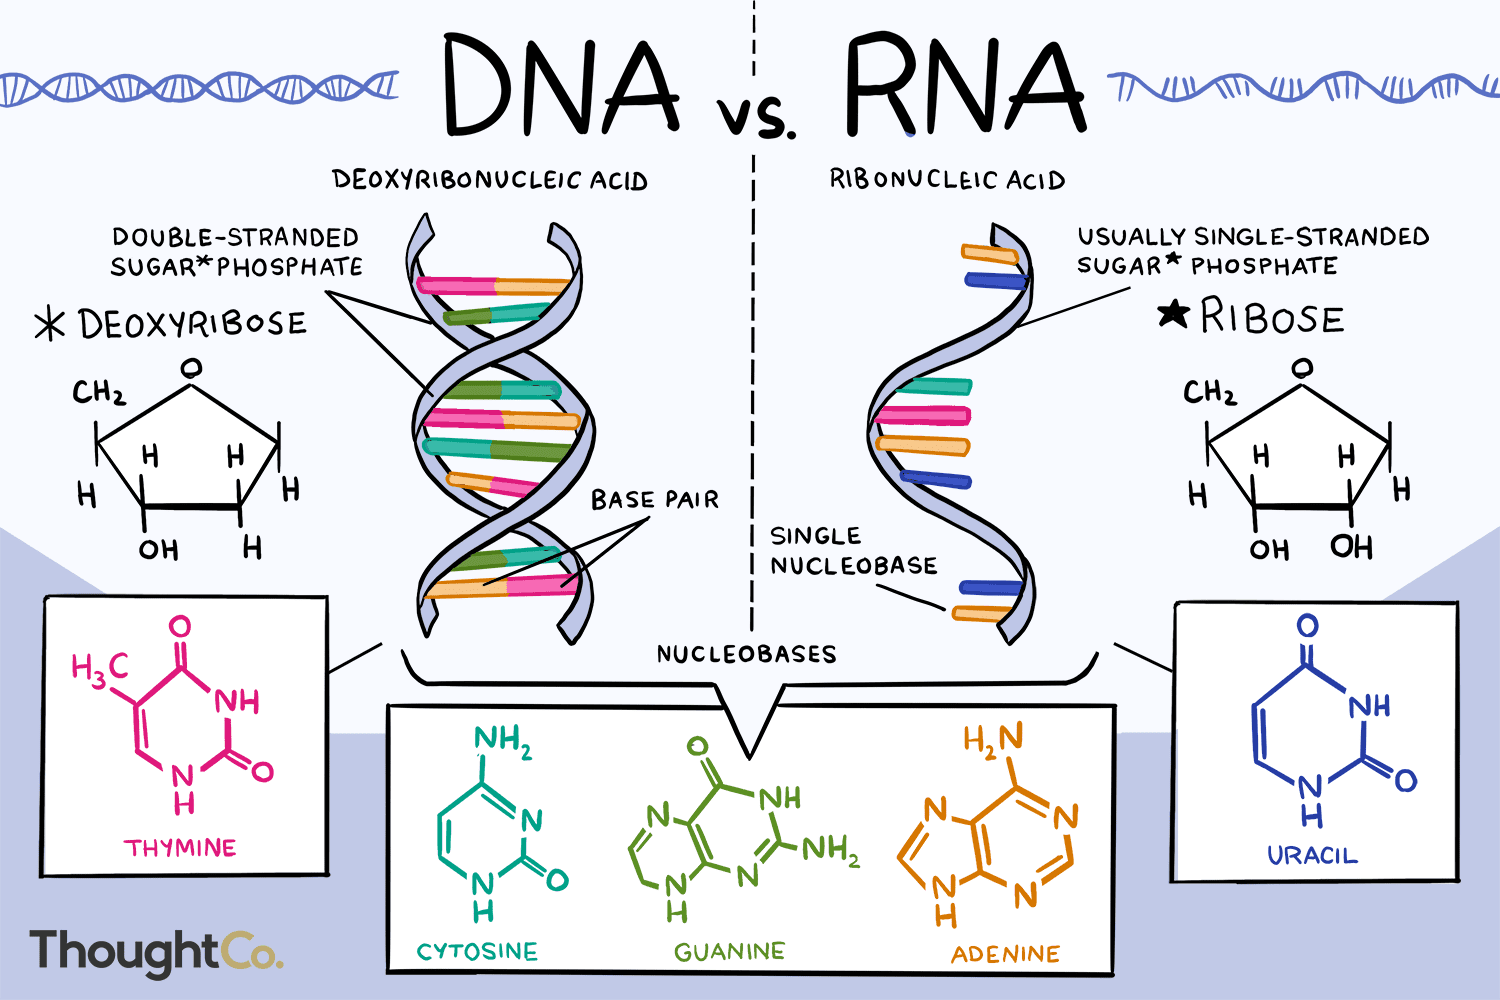
\includegraphics[width=10cm, ]{pictures/dnarna.png}
\caption{
مقایسه دی‌ان‌ای و آران‌ای
}\label{wrap-fig:3}
\end{wrapfigure}

شباهت‌ها:
\begin{itemize}
\item هر دو پلیمر هستند و از نوکلئوتید تشکیل شده‌اند.
\item در هر دو نوکلئوتیدهای مقابل با پیوند هیدروژنی و نوکلئوتیدهای کناری با پیوند فسفو دی‌استر به هم متصل می‌شوند (گاهی نوکلئوتیدهای دو بخش متفاوت از یک رشته آران‌ای، به هم متصل می‌شوند).
\item نوکلئوتیدهای آزاد (واحدهای سازنده آزاد) هر دو مولکول پیش از اتصال سه فسفات بوده و با اتصال به رشته پلی‌نوکلئوتیدی تک‌فسفاته می‌شوند.

\end{itemize}}

\newpage

\section{ویرایش ژنوم}
مهندسی ژنوم یا ویرایش ژنوم نوعی از مهندسی ژنتیک است که در آن دی‌ان‌ای ژنوم یک موجود زنده حذف، اضافه، اصلاح یا جایگزین می‌شود. در دهه ۱۹۶۰، دانشمندان با شارش پرتو‌های رادیواکتویی بر روی گیاهان دست به تغییر ژنوم‌ آنها به طور کاملا تصادفی زندند. این کار به هدف رسیدن به یک تغییر ژنتیک مفید صورت می‌گرفت و البته نتابج خوبی هم به همراه داشت ولی با این حال راندمان پایین این ویرایش‌ها باعث شد که دانشمندان به فکر راه‌های دیگری برای ویرایش ژنوم باشند.

تا کنون سه تکنیک موفق و معروف برای ویرایش ژنوم مهندسی شده است:
 نوکلئاز انگشت روی\LTRfootnote{\lr{Zinc Finger Nuclease}} 
\lr{(ZFNs)}
، نوکلئازهای اثرگذار شبه فعال کننده رونویسی\LTRfootnote{\lr{Transcription activator-like effector nuclease}} 
\lr{(TALEN)}
، و سیستم تناوب‌هایِ کوتاهِ پالیندرومِ فاصله‌دارِ منظمِ خوشه‌ای\LTRfootnote{\lr{Clustered Regularly Interspaced Short Palindromic Repeats}}
\lr{(CRISPR)}. 
کلید ویرایش ژنوم ایجاد شکست دو رشته‌ی DNA در نقطه مورد نظر است و این سه روش مبتنی بر شکست درست DNA در نقطه مورد نظر مهندسی شدند.
\subsection{ شکست و تعمیر دی‌ان‌ای}

شکل رایج ویرایش ژنوم بر مفهوم مکانیک ترمیم شکست دو رشته‌ای DNA
\LTRfootnote{\lr{Double-Strand Break (Cut)}}\lr{(DSB)}
تکیه دارد. دو مسیر اصلی وجود دارد که DSB را تعمیر می‌کند. اتصال انتهای غیر همولوگ
\LTRfootnote{\lr{Non-Homologous End Joining}}
 \lr{(NHEJ)}
  و تعمیر هدایت شده همولوژی
 \LTRfootnote{\lr{Homology Directed Repair}}
   \lr{(HDR)}. NHEJ از انواع آنزیم‌ها برای اتصال مستقیم به انتهای DNA استفاده می‌کند، در حالی که HDR دقیق‌تر از یک توالی همولوگ به عنوان الگویی برای بازسازی توالی‌های DNA گمشده در نقطه شکست استفاده می‌کند. این را می توان با ایجاد یک بردار با عناصر ژنتیکی مورد نظر در یک توالی که همولوگ با توالی های کناری یک DSB است مورد استفاده قرار داد. این باعث می شود که تغییر مورد نظر در محل DSB درج شود. در حالی که ویرایش ژن مبتنی بر HDR مشابه هدف‌گیری ژن مبتنی بر نوترکیب همولوگ است، نرخ نوترکیبی حداقل سه مرتبه افزایش می‌یابد.

\subsubsection{NHEJ}
\begin{wrapfigure}{l}{9cm}
\centering
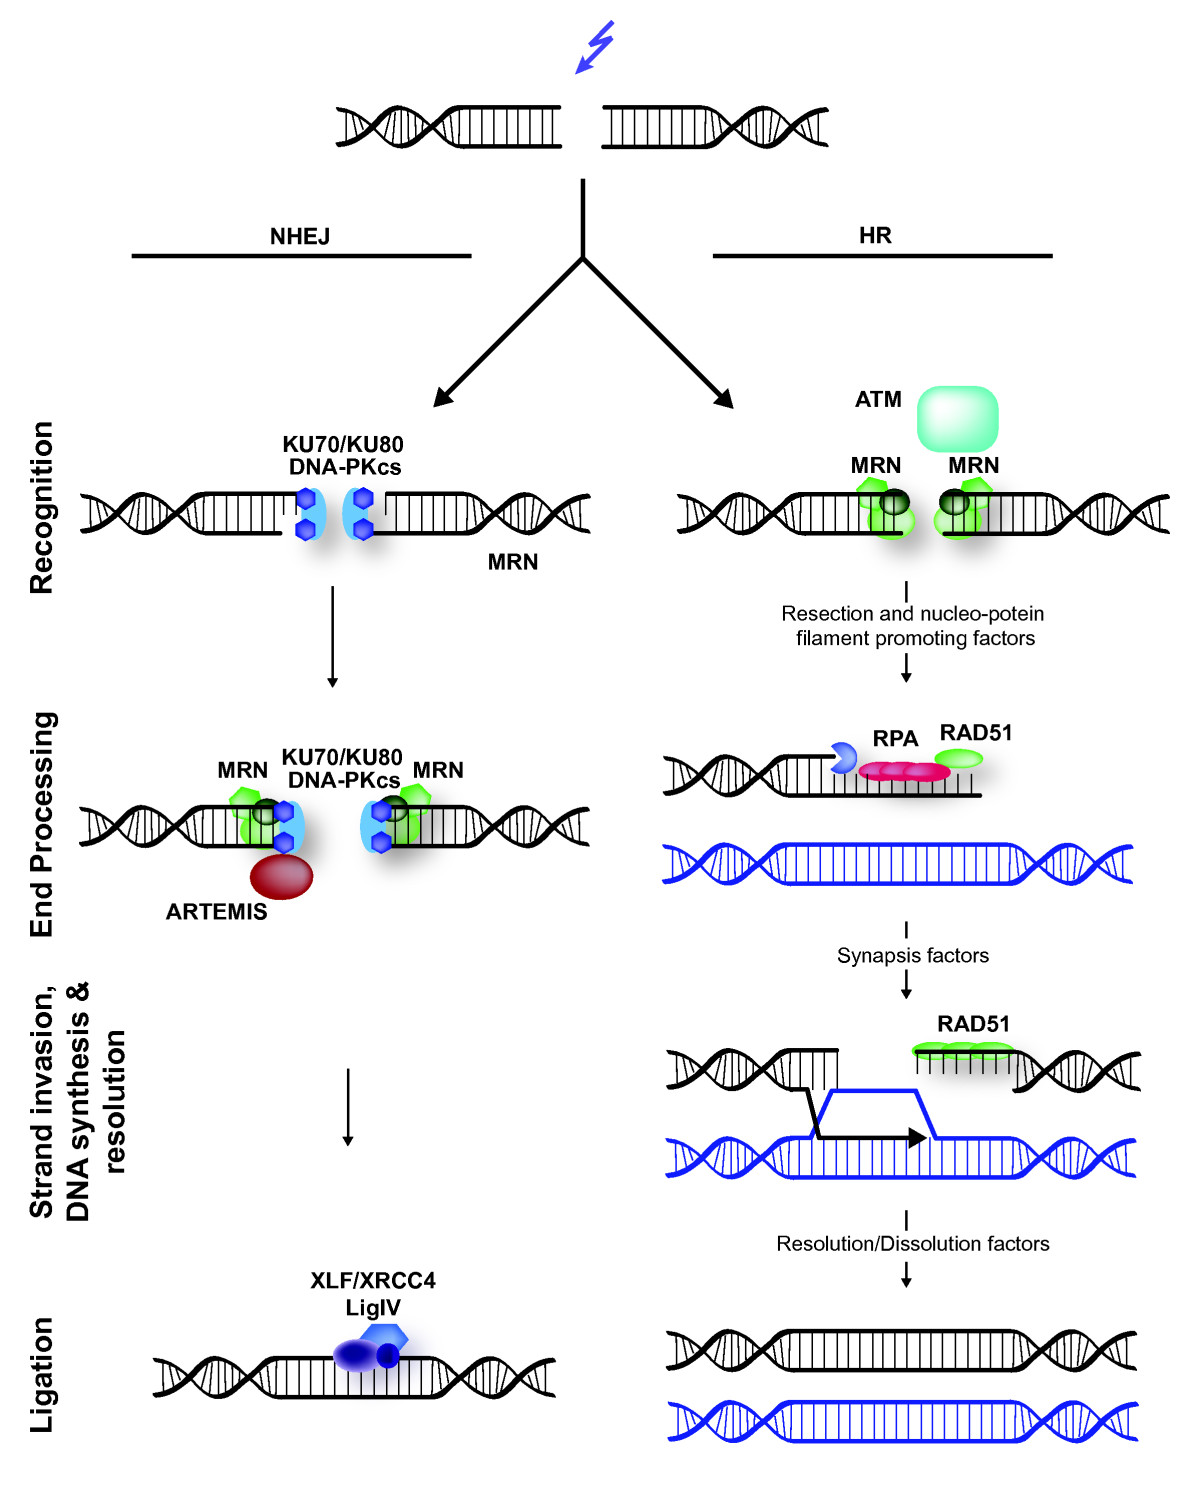
\includegraphics[width=8cm, ]{pictures/DBSrepair.jpg}
\caption{
مکانیزم ترمیم DNA
}\label{wrap-fig:4}
\end{wrapfigure}
پرتوهای یونیزه کننده و برخی داروهای ضد سرطان باعث شکست هر دو رشته ی DNA می شوند .سیستمی که برای ترمیم این نوع آسیب به کار گرفته میشود، سیستم ترمیم اتصال انتهای غیر همولوگ (NHEJ) میباشد که مستعد به خطا به شمار می رود، زیرا همواره چندین نوکلئوتید در جایگاه ترمیم از بین می روند و دو انتهای شکسته شده از کروموزوم های همولوگ یا غیر همولوگ به یکدیگر متصل می شوند.
زمانی که کروماتیدهای خواهری برای ترمیم شکست های دو رشته ای در دسترس نباشند این نوع ترمیم صورت میگیرد . در ابتدا کمپلکسی از ku70/80 و پروتئین کیناز وابسته به DNA به انتهاهای شکسته دو رشته اتصال می یابند، آن گاه در هر انتها چندین باز توسط نوکئاز حذف شده و دو مولکول از طریق آنزیم لیگاز به هم متصل می گردند. 
\lr{DSB}ها
 ترجیحاً در سلول توسط اتصال انتهایی غیر همولوگ (NHEJ) ترمیم می شوند، مکانیزم سریعی که اغلب باعث درج یا حذف (indels) در DNA می شود. ایندل ها اغلب منجر به تغییر اساسی در DNA می شوند و به‌طوری که DNA عملکرد خود را از دست می دهند. پس در نتیجه معمولا به عنوان سلول مرده درنظر گرفته میشوند و حذف می‌شوند. برای ویرایش ژنوم مطمئن اعمال شدن ویرایش و تغییر نکردن آن نکته مهمی است. پس دانشمندان تمام تلاششان را میکنند که بعد از DBS، DNA به این روش تعمیر نشود.

\newpage
\subsubsection{HDR}
 تعمیر هدایت شده همولوژی (HDR) مکانیزمی در سلول ها برای ترمیم ضایعات DNA دو رشته‌ای از یک نسخه مشابه DNA برای ترمیم استفاده می کند. رایج ترین شکل HDR نوترکیبی همولوگ است. مکانیسم HDR تنها زمانی می تواند توسط سلول استفاده شود که یک قطعه همولوگ از DNA در هسته وجود داشته باشد، عمدتاً در فاز G2 و S چرخه سلولی. نمونه‌های دیگر تعمیر مبتنی بر HDR شامل تعمیر تک رشته‌ای و تکثیر ناشی از شکستگی است. هنگامی که DNA همولوگ وجود ندارد، فرآیند NHEJ به جای آن انجام می‌شود.

\subsection{\lr{Zinc finger nucleases (ZFN)}}

نوکلئاز انگشت روی یا ZFN اولین سیستم پروتئینی متصل شونده به DNA قابل برنامه ریزی با کاربرد وسیع است.ZFNها شامل زنجیره ای از پروتئین های انگشت روی هستند که به یک نوکلئاز باکتریایی ملحق شده اند تا بتوانند سیستمی را تولید کنند که قادر به ایجاد برش های دو رشته ای خاص در DNA برای ویرایش ژن باشد. پروتئین های انگشت روی هدف قرار دادن ناحیه خاص را فراهم می کنند زیرا هر یک از آنها سه جفت باز یا ۳bp از DNA را شناسایی می کنند. نوکلئازی که معمولاً در تکنولوژی ZFN متصل به زنجیره پروتئین های انگشت روی است FokI نام دارد که برای اتصال به DNA باید دایمریزه شده باشد، بنابراین یک جفت از ZFN برای هدف گیری و برش DNA مورد استفاده قرار می گیرد.این آنزیم ها کمک زیادی به تولید موجودات ترانسژنیک می کنند و بدلیل اینکه فراوانی نوترکیبی همولوگ بسیار ناچیز بوده اهمیت زیادی در مهندسی ژنتیک و مطالعات ترانسژنیک ، ناک اوت و غیره پیدا کرده اند. این پروتئین های مهندسی شده متصل شونده به DNA می توانند ژنوم را در جایگاه های ویژه ای شناسایی کرده و ایجاد برش های دورشته ای کنند . در صورتیکه سیستم تعمير NHEJ فعال شود چون این سیستم ترمیم مستعد خطاست سبب ایجاد جهش در آن ناحیه خاص از ژنوم می شود بنابراین در مطالعات موتاژنز نیز اهمیت دارند. انتقال یک وکتور حاوی ژن مورد نظر به همراه ZFNs سبب تسهیل درج ژن در آن ناحیه از ژنوم می گردد.

\subsection{TALEN}
\begin{wrapfigure}{l}{8cm}
\centering
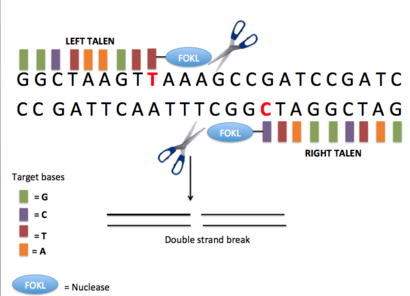
\includegraphics[width=8cm, ]{pictures/Overview_of_TALENs.png}
\caption{
مکانیزم TALEN
}\label{wrap-fig:4}
\end{wrapfigure}
نوکلئازهای رونویس مؤثر-مانند فعال‌کننده
 \lr{(TALENs)}
 پروتئین‌های خاصی هستند که به DNA متصل می‌شوند که دارای آرایه‌ای از 33 یا 34 تکرار  آمینه اسیدها هستند. 
\lr{TALEN}
ها آنزیم های محدودکننده مصنوعی هستند که با ادغام حوزه برش DNA یک نوکلئاز با دامنه های TALE طراحی شده اند، که می توانند به طور خاص یک توالی DNA منحصر به فرد را شناسایی کنند. این پروتئین‌های ادغام شده به‌عنوان قیچی DNA به‌راحتی قابل برنامه‌نویسی برای ویرایش یک ژن خاص عمل می‌کنند که قادر به انجام تغییرات هدفمند ژنوم مانند درج توالی، حذف، تعمیر و جایگزینی در سلول‌های زنده هستند. این تکنولوژی را می‌توان برای تغییر هر نقطه از DNA استفاده کرد.
 \lr{TAL‌}های
 موثر یک رشته ۳۴تایی از آمینو‌اسید‌ها هستند که هر کدام وظیفه دارند یک تک نوکلئوتید را پیدا کنند. نوکلئاز می‌تواند شکستگی‌های دو رشته‌ای را در محل هدف ایجاد کند که می تواند با اتصال انتهایی غیر همولوگ (NHEJ) ترمیم شود، که منجر به اختلالات ژنی از طریق وارد کردن یا حذف های کوچک می شود. هر تکرار حفظ می شود، به جز آمینواسید ۱۳ و ۱۲ که به آنها دو باقیمانده متغیر تکرار (RVDs) می‌گویند. RVD ها توالی DNA را تعیین می کنند که TALE به آن متصل می شود. این تناظر ساده یک به یک بین تکرارهای TALE و توالی DNA مربوطه باعث می‌شود روند مونتاژ آرایه‌های تکراری برای تشخیص توالی‌های DNA جدید ساده باشد. این 
\lr{TALE}ها
 را می توان با کاتالیزوری از یک نوکلئاز از DNA به نام FokI، ادغام کرد تا با آن TALENها را ساخت. ساختارهای TALEN توالی‌های DNA را فقط در مکان‌های از پیش انتخاب شده متصل می‌کنند و می‌شکنند. هدف TALEN را می توان بر اساس یک کد آسان پیش بینی کرد. نوکلئازهای TAL تا حدی به دلیل طولشان که بیش از 30 جفت است میتوان فقط مختص آن هدف درنظر گرفت. TALEN را می توان در محدوده 6 جفت باز از هر نوکلئوتید منفرد در کل ژنوم انجام داد.

سازه های TALEN به روشی مشابه با نوکلئازهای انگشت روی طراحی شده استفاده می‌شوند و دارای سه مزیت در جهش زایی هدفمند هستند: (1) اختصاصیت اتصال به DNA بالاتر است، (2) اثرات خارج از هدف کمتر است و (3) طراحی آن آسان تر است.
\newpage
\section{CRISPR}
 \lr{Clustered Regularly Interspaced Short Palindromic Repeats}
) یا به اختصار کریسپر (به انگلیسی: CRISPR) به معنی "تناوب‌هایِ کوتاهِ پالیندرومِ فاصله‌دارِ منظمِ خوشه‌ای" بخشی از دی‌ان‌ای پروکاریوت هستند که حاوی تناوب‌های کوتاهِ توالی‌های بنیادین هستند. بخشی از سیستم کریسپر "پروتئین Cas9" است. این پروتئین قابلیت جستجو، برش زدن و تغییر دی ان ای(DNA) را دارد. قبل از این تکنیک از روش "تحویل یا انتقال ژن" استفاده می‌شد، به این صورت که از یک ناقل ویروسی یا غیرویروسی برای انتقال ژن سالم به ژنوم سلول میزبان استفاده می‌شد، ولی در روش کریسپر، ژن معیوب برش داده می‌شود و ژن سالم به جای آن قرار می‌گیرد. استفاده از آنزیم Cas9 خطر کمتری نسبت به روش قبلی که یک ژن خارجی وارد ژنوم می‌شد دارد، زیرا گاهی ژن خارجی به سرطان منجر می‌شود اما ژنی که از طریق کریسپر ترمیم شود کنترل شده است. نام دیگر این تکنیک "قیچی ژنتیکی" است که به دلیل ساز و کار آنزیم "کَس9" (Cas9) هست. این آنزیم به عنوان یک جفت قیچی مولکولی می‌تواند دو رشته DNA را در محل خاصی از ژنوم برش دهد.[۱]
\begin{figure}[!h]
\centering
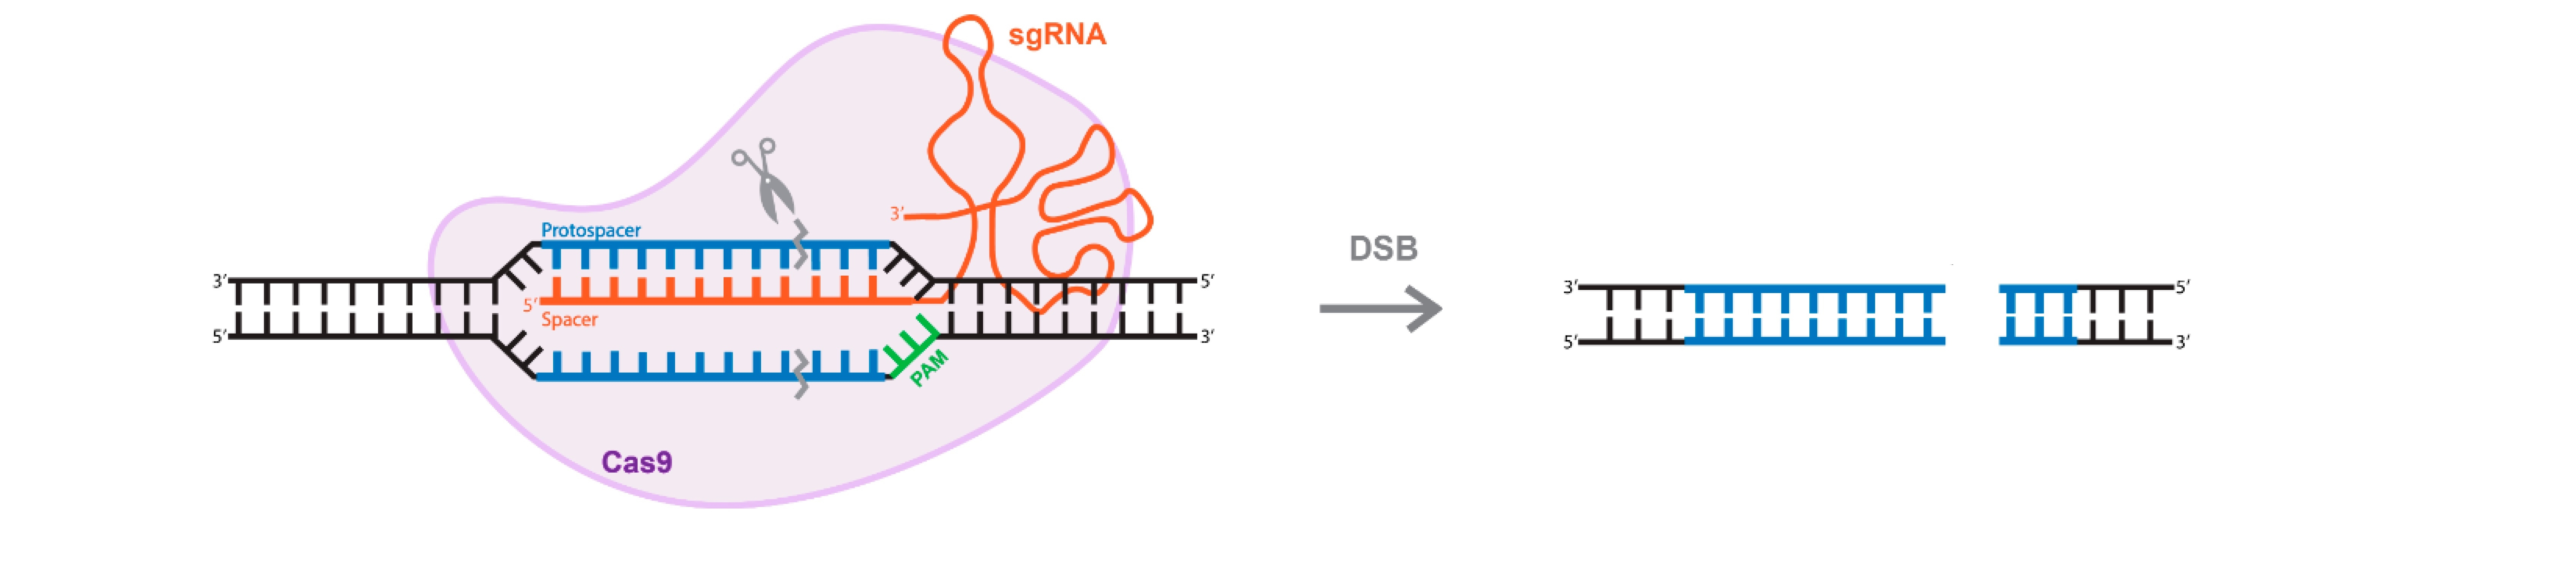
\includegraphics[width=10cm, ]{pictures/simple_crispr.jpg}
\caption{
مکانیزم ساده شده‌ای از CRISPR
}\label{fig:1}
\end{figure}

\subsection{کریسپر در باکتری}

اولین بار سیستم کریسپر در
 \lr{Escherichia coli}
 به عنوان یک توالی تکراری ۲۹ نوکلئوتیدی با فاصله ۳۲ نوکلئوتیدی توسط یوشیزومی ایشی نو ژاپنی در سال ۱۹۸۷ مطرح شد که باکتری‌ها و آرکی باکتری‌ها را از حمله باکتریوفاژها و پلاسمیدها محافظت می‌کند. این سیستم‌های دفاعی به یک RNA کوچک شناساگر توالی خاص تکیه می‌کنند و اسیدهای نوکلئیک خارجی را خاموش می‌کنند.
[۲] \lr{Francisco Mojica}
 و همکارانش در سال ۱۹۹۳ تکرارهای مشابهی را در چندین گونه میکروبی دیگر یافتند.[۳]
بعد از حمله به سلول توسط عناصر ژنتیکی خارجی مانند باکتریوفاژها یا پلاسمیدها (مرحله ۱: تزریق فاژ)، آنزیم‌های ویژه مرتبط CRISPR
 به نام
 \lr{Cas (CRISPR-associated protein)}
 توالی‌های spacer را از توالی‌های protospacer جدا کرده و آن‌ها را به درون لوکوس‌های کریسپر موجود در ژنوم پروکاریوت‌ها وارد و متصل می‌کنند. (مرحله ۲: استفاده از spacer). این 
\lr{spacer}ها
 بین تکرارهای مستقیم تقسیم شده‌اند که اجازه می‌دهند سیستم CRISPR، به‌طور ایمن و دقیق و نه به‌طور غیر ایمن شناسایی شود. آرایهٔ CRISPR یک رونوشت RNA غیر کدونی است که از نظر آنزیمی از طریق مسیرهای متمایز که برای هر نوع سیستم CRISPR منحصر به فرد است، بالغ می‌شود. (مرحله ۳: بیوژنز و پرادازش CrRNA) در CRISPR نوع I و
 \lr{،III} 
رونوشت pre-CrRNA توسط ریبونوکلئازهای مرتبط با CRISPR، شکسته می‌شوند و این کار موجب آزاد شدن چندین CrRNAs کوچک می‌شود. به‌طور متوسط CrRNA نوع III بیشتر در انتهای ´۳ توسط
 \lr{RNase}هایی 
که هنوز مشخص نشده‌اند برای تولید رونوشت کاملاً بالغ پردازش می‌شوند. CRISPR نوعII، یک RNA کریسپر فعال‌کننده ترانس است (tracrRNA) که با تکرارهای مستقیم هیبرید می‌شود و یک RNA دوپلکس را تشکیل می‌دهد و توسط 
\lr{RNase III}
 درونی و نوکلئازهای ناشناخته دیگر شکسته و پردازش می‌شود. CrRNAهای بالغ شده نوع I و III سیستم CRISPR، سپس درون افکتورهای کمپلکس‌های پروتئینی برای تشخیص و تخریب توالی هدف اضافه می‌شوند. در سیستم‌های نوع II، کمپلکس هیبرید CrRNA-tracrRNA به Cas9 متصل شده و در واقع هیبرید شدن این دو باعث فعال شدن Cas9 می‌شود. هر دو نوع I و III سیستم CRISPR از چند پروتئین مداخله گر تنظیم‌کننده برای تسهیل شناسایی توالی هدف استفاده می‌کنند. در CRISPR نوعI، کمپلکس Cascade با یک مولکول CrRNA لود می‌شود که یک مجموعه نظارتی بی نظیری است که DNA هدف را شناسایی می‌کند. سپس نوکلئازCas3، لوپ R Cascade را به کار گرفته و به آن متصل می‌شود و واسطه تخریب توالی هدف می‌شود. در CRISPR نوع III, CrRNAها یا به کمپلکس‌های Csm یا به کمپلکس‌های Cmr به ترتیب متصل شده و به ترتیب سوبستراهای DNA و RNA را می‌شکنند. درمقابل، سیستم نوع II فقط نیاز به Cas9 برای تخریب DNA جفت شده با RNA راهنما دوپلکس خود دارد که این RNA راهنما حاوی ترکیبی از CrRNA-tracrRNA است.[۵]
\subsection{عمل کرد کریسپر در ژن}
همانطور که گفتیم، مدل‌های مختلفی از CRISPR تا به حال درست شده است ولی به صورت کلی می‌توان CRISPR را به دو قسمت RNA و  cas تقسیم کرد که cas در آن وظیفه جدا کردن دو رشته DNA را از هم دارد و RNA که هدف را مشخص و قیچی می‌کند. برای این که دقیقا نقطه شکست DNA مشخص شود cas نیاز به یک سیگنال است که با رسیدن به آن کار خود را شروع کند. به این رشته PAM یا 
\lr{Protospacer Adjacent Motif}
گفته می‌شود که کاملا وابسته به cas است. همان طور که از قبل گفتیم بعد از شکست DNA، دو مکانیزم برای تعمیر آن وجود دارد. دانشمندان تکنولوژی‌های CRISPR مختلفی را برای افزایش احتمال تعمیر HDR ایجاد کرده‌اند که با که هر یک ویژگی‌های خاص خود را دارند ولی ما در پژوهش خود ساده‌ترین مورد آن یعنی cas9 به همراه یک RNA که به آن sgRNA یا 
\lr{single guide RNA}
می گویند، استفاده کرده‌ایم. این طرح باعث محدود شدن هدف‌های مورد استفاده می‌شود به طوری که ‌PAM باید به شکل NGG باشد که در آن N یک نوکلیوتید دلخواه است. در نتیجه رشته هدف همیشه با NGG ختم میشود. 
\begin{figure}[!h]
\centering
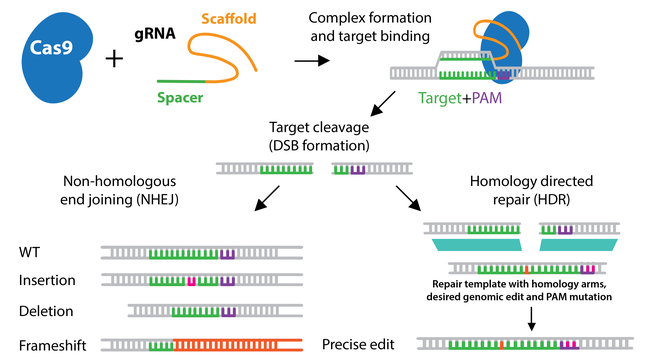
\includegraphics[width=12cm, ]{pictures/cut.png}
\caption{
مکانیزم CRISPR
}\label{fig:2}
\end{figure}
 
\subsection{حساسیت}
حساسیت در یک طرح CRISPR میزان اختصاصی بودن توالی هدف گیری شده توسط gRNA در مقایسه با بقیه ژنوم تعیین می شود. در حالت ایده‌آل، یک توالی هدف‌گیری شده توسط gRNA همسانی کاملی با DNA هدف خواهد داشت و هیچ همسانی در جای دیگری در ژنوم وجود ندارد یعنی دقیقا هدف را ویرایش می‌دهد نا جای دیگری را. با این حال، به طور واقع بینانه، یک توالی که با gRNA هدف قرار گرفته شده، مکان‌های بیشتری در سراسر ژنوم ویرایش خواهد داد که در آن همولوژی نسبی وجود دارد. این ناحیه‌ها خارج از هدف یا offtarget نامیده می شوند و باید هنگام طراحی یک gRNA برای آزمایش خود در نظر گرفته شوند.

علاوه بر بهینه سازی طراحی gRNA، حساسیت CRISPR نیز می تواند از طریق تغییرات در Cas9 افزایش یابد. همانطور که قبلاً بحث شد، Cas9 از طریق فعالیت ترکیبی دو حوزه نوکلئاز، RuvC و HNH، شکست‌های دو رشته ای (DSBs) ایجاد می کند. نیکاز Cas9، یک جهش D10A از SpCas9، یک دامنه نوکلئاز را حفظ می‌کند و به جای DSB، یک DNA نیک تولید می کند.

بنابراین، دو نیکاز که رشته‌های DNA مخالف را هدف قرار می دهند برای تولید DSB در DNA هدف مورد نیاز است. این نیاز برای یک سیستم CRISPR نیکاز دوتایی یا نیکاز دوگانه به طور چشمگیری ویژگی هدف را افزایش می‌دهد، زیرا بعید است که دو ناک خارج از هدف به اندازه کافی نزدیک به ایجاد DSB ایجاد شوند. اگر حساسیت بالا برای آزمایش شما بسیار مهم است، ممکن است استفاده از رویکرد نیکاز دوگانه را برای ایجاد یک DSB القا شده با نیک دوگانه در نظر بگیرید. سیستم نیکاز همچنین می تواند با ویرایش ژن با واسطه HDR برای ویرایش های ژنی خاص ترکیب شود.

در سال 2015، محققان از 
\lr{rational mutagenesis}
 برای توسعه دو Cas9 با ثبات بالا استفاده کردند:
\lr{eSpCas9} و\lr{SpCas9-HF1}.   
 \lr{eSpCas9} حاوی جایگزین‌های آلانین است که برهمکنش‌های بین شیار HNH/RuvC و رشته DNA غیرهدف را تضعیف می‌کند و از جدا شدن رشته‌ها و برش در مکان‌های خارج از هدف جلوگیری می‌کند. به طور مشابه، SpCas9-HF1 ویرایش خارج از هدف را از طریق جایگزینی آلانین کاهش می دهد که برهمکنش Cas9 با ستون فقرات فسفات DNA را مختل می کند. یکی دیگر از Cas9 با وفاداری بالا، HypaCas9، در سال 2017 توسعه یافت و حاوی جهش‌هایی در دامنه REC3 است که تصحیح Cas9 و تبعیض هدف را افزایش می‌دهد. هر سه آنزیم با وفاداری بالا نسبت به Cas9 نوع وحشی ویرایش خارج از هدف کمتری تولید می کنند.

\subsection{تاثیرگذاری}
تاثیرگذاری در یک طرح CRISPR احتمال شکست DNA و ویرایش درست را تعیین ‌می‌کند. برای غلبه بر راندمان پایین HDR، محققان دو دسته از ویرایشگرهای پایه را ایجاد کرده‌اند - ویرایشگرهای پایه سیتوزینی \lr{(CBEs)} و ویرایشگرهای پایه آدنین \lr{(ABEs)}.

ویرایشگرهای پایه سیتوزینی با ادغام نیکاز Cas9 یا Cas9 مرده غیرفعال کاتالیزوری \lr{(dCas9)} به سیتیدین دآمیناز مانند APOBEC ایجاد می‌شوند. ویرایشگرهای پایه توسط یک gRNA به یک مکان خاص قرار می‌گیرند و می توانند سیتیدین را در یک پنجره ویرایش کوچک در نزدیکی سایت PAM به یوریدین تبدیل کنند. اوریدین متعاقباً از طریق ترمیم برش پایه به تیمیدین تبدیل می‌شود و تغییر C به T (یا G به A در رشته مخالف) ایجاد می‌کند.

به طور مشابه، ویرایشگرهای پایه آدنوزین برای تبدیل آدنوزین به اینوزین مهندسی شده‌اند، که سلول با آن مانند گوانوزین رفتار می‌کند و تغییر A به G (یا T به \lr{(C} ایجاد می‌کند. آدنین DNA دآمینازها در طبیعت وجود ندارند، اما با تکامل هدایت شده \lr{Escherichia coli TadA}، یک tRNA آدنین دآمیناز ایجاد شده اند. مانند ویرایشگرهای پایه سیتوزین، دامنه تکامل یافته TadA با پروتئین Cas9 ترکیب می شود تا ویرایشگر پایه آدنین ایجاد شود.

هر دو نوع ویرایشگر پایه با چندین نوع Cas9 از جمله Cas9 با ثبات بالا در دسترس هستند. پیشرفت‌های بیشتری با بهینه‌سازی بیان پروتئین، اصلاح ناحیه پیوندی بین نوع Cas و دآمیناز برای تنظیم پنجره ویرایش، یا افزودن ترکیب‌هایی که خلوص محصول را افزایش می‌دهند مانند مهارکننده DNA گلیکوزیلاز \lr{(UGI)} یا Gam مشتق از باکتریوفاژ \lr{(Mu-GAM)} انجام شده است.






\subsection{انواع کریسپر}
طبقه‌بندrova و همکاران ۵ نوع سیستم کریسپر را تعریف می‌کند که دارای ۱۶ زیر نوع بر اساس ویژگی‌های مشترک و شباهت تکاملی است. اینها به دو دسته بزرگ تقسیم می‌شوند. کلاس‌ها بر اساس ساختار پیچیده‌ای است که DNA ژنوم را تجزیه می‌کند. نوع II CRISPR/Cas اولین سیستم برای مهندسی ژنوم، با نوع V در ۲۰۱۵ بود.[۴]

در گام بعدی از روی ژن‌های کمپلکس cas هم پروتئین Cas9 ساخته می‌شود. سپس کمپلکس Cas9-crRNA-tracrRNA تشکیل می‌شود؛ که این کمپلکس لازم و ضروری برای هدف قرار دادن یا تخریب DNAخارجی می‌باشد.

\subsubsection{ Single-Strand Break (Nick)}
\begin{wrapfigure}{l}{8cm}
\centering
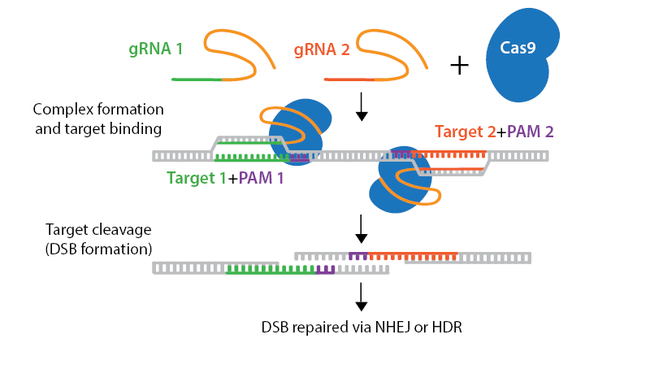
\includegraphics[width=8cm, ]{pictures/nick.png}
\caption{
مکانیزم TALEN
}\label{wrap-fig:4}
\end{wrapfigure}
در حالی که بسیاری از ویرایشگرهای پایه برای کار در یک پنجره بسیار نزدیک به دنباله PAM طراحی شده‌اند، برخی از سیستم‌های ویرایش پایه طیف گسترده‌ای از انواع تک نوکلئوتیدی \lr{(somatic hypermutation)} را در یک پنجره ویرایش گسترده‌تر ایجاد می‌کنند و بنابراین برای تکامل هدایت‌شده مناسب هستند. برنامه های کاربردی. نمونه‌هایی از این سیستم‌های ویرایش پایه عبارتند از جهش‌زایی هدفمند با واسطه \lr{AID (TAM)} و \lr{CRISPR-X}، که در آن Cas9 با سیتیدین دآمیناز \lr{(AID)} ناشی از فعال‌سازی ترکیب می‌شود.

نیکاز \lr{CRISPR/Cas} جهش‌یافته‌، به‌جای شکستگی‌های دو رشته‌ای ایجاد شده توسط آنزیم‌های Cas، شکستگی‌های تک‌رشته‌ای با هدف gRNA را در DNA ایجاد می‌کنند. برای استفاده از جهش نیکاز، به دو gRNA نیاز دارید که رشته‌های مخالف DNA شما را در مجاورت یکدیگر مورد هدف قرار دهند. این شیارهای دوتایی یک شکست دو رشته ای (DSB) ایجاد می کنند که با استفاده از اتصال انتهایی غیر همولوگ \lr{(NHEJ)} و مستعد خطا تعمیر می شود. استراتژی‌های دوتایی اثرات ناخواسته off-targets را کاهش می‌دهند. جهش‌یافته‌های نیکاز همچنین می‌توانند با یک الگوی تعمیر برای معرفی ویرایش‌های خاص از طریق تعمیر هدایت‌شده همولوژی \lr{(HDR)} استفاده شوند.

در حالی که \lr{S. pyogenes Cas9} (SpCas9) مطمئناً متداول ترین اندونوکلئاز CRISPR برای مهندسی ژنوم است، ممکن است بهترین اندونوکلئاز برای هر کاربرد نباشد. به عنوان مثال، توالی PAM برای SpCas9 (5'-NGG-3') در سراسر ژنوم انسان فراوان است، اما یک توالی NGG به درستی برای هدف قرار دادن ژن‌های مورد نظر برای اصلاح قرار نگیرد. این محدودیت در هنگام تلاش برای ویرایش یک ژن با استفاده از تعمیر هدایت‌شده همولوژی (HDR)، که نیاز به توالی‌های PAM در مجاورت بسیار نزدیک به منطقه برای ویرایش دارد، نگران کننده است.

برای رسیدگی به این محدودیت‌ها، محققان آنزیم‌های SpCas9 را با ویژگی‌های تغییر یافته PAM با استفاده از روش‌های مختلفی از جمله تکامل به کمک فاژ و جهش‌زایی هدایت‌شده مهندسی کرده‌اند. این منجر به توسعه چندین نوع مشتق شده از SpCas9 با توالی های PAM غیر NGG شد. جایگزین دیگر \lr{،Cas9}  xCas9 است که مجموعه وسیعی از توالی های PAM مانند \lr{NG ،GAA} و GAT را هدف قرار می دهد، در حالی که حداقل فعالیت خارج از هدف را نیز نشان می دهد.

\begin{table}[!ht]
    \centering
    \begin{tabularx}{\textwidth}{|r|X|}
    	\rowcolor{Goldenrod}	
        اصطلاح & تعریف \\ \hline
       ویرایشگر پایه \lr{(Base editor)}
 & ادغام یک پروتئین Cas به یک دآمیناز که تبدیل مستقیم باز در RNA یا DNA را بدون شکست دو رشته DNA امکان پذیر می کند.\\ \hline
        \lr{Cas} & \lr{CRISPR Associated Protein,} شامل نوکلئازهایی مانند Cas9 و Cas12a (همچنین به عنوان Cpf1 شناخته می شود) \\ \hline
        \lr{CRISPR} & تناوب‌هایِ کوتاهِ پالیندرومِ فاصله‌دارِ منظمِ خوشه‌ای، یک منطقه ژنومی باکتریایی که در دفاع از پاتوژن استفاده می شود \\ \hline
        \lr{CRISPRa} & \lr{CRISPR Activation;} استفاده از فعال کننده dCas9 یا dCas9 با gRNA برای افزایش رونویسی یک ژن هدف\\ \hline
        \lr{CRISPRi} & \lr{CRISPR Interference;}
 استفاده از dCas9 یا dCas9-سرکوبگر با gRNA برای مانع/کاهش رونویسی یک ژن هدف \\ \hline
        برش & شکستن دو رشته ای DNA \\ \hline
        \lr{dCas9} & \lr{Nuclease dead Cas9,} شکل آنزیمی غیر فعال Cas9. می تواند متصل شود، اما نمی تواند DNA را بشکند \\ \hline

جفت نیکاز یا نیک دوتایی & روشی برای کاهش اثرات خارج از هدف با استفاده از یک نیکاز Cas9 و 2 gRNA  \\
\lr{(Dual nickase/Double nick)}
& مختلف که در مجاورت رشته های مخالف DNA متصل می شوند تا یک DSB ایجاد کنند. \\ \hline

اصلاح یا ویرایش ژنتیکی &  هر گونه اختلال ژنتیکی، از جمله حذف ژنتیکی، فعال سازی ژن، یا سرکوب ژن \\      
 \lr{(Genetic modification or manipulation)} & \\ \hline
        \lr{gRNA} & \lr{Guide RNA,}
 باکتریایی درون‌زا که از ادغام مصنوعی crRNA و tracrRNA به وجود می‌آید که هم هدف و هم امکان چسبیدن به Cas9 فراهم می‌کند. این ادغام مصنوعی در طبیعت وجود ندارد و معمولاً به آن sgRNA نیز می‌گویند.
         \\ \hline
        \lr{gRNA scaffold sequence} &
 توالی درون gRNA که مسئول اتصال به Cas9 است، شامل توالی spacer/هدف 20 جفت باز که برای هدایت Cas9 به DNA هدف استفاده می‌شود، نمی‌شود.\\ \hline
        \lr{gRNA targeting sequence} & 
۲۰ نوکلئوتید قبل از توالی PAM در DNA ژنومی قرار دارند. این توالی در یک پلاسمید بیان gRNA کلون می شود اما شامل توالی PAM یا توالی scafold gRNA نمی شود. \\ \hline
        \lr{HDR} & \lr{Homology Directed Repair}, یک مکانیسم ترمیم DNA که از یک الگو برای ترمیم نیک های DNA یا DSB ها استفاده می کند \\ \hline
       ایندل \lr{(Indel)} & \lr{Insertion/deletion}, نوعی جهش که می تواند منجر به اختلال در یک ژن با جابجایی ORF و/یا ایجاد کدون های توقف زودرس شود. \\ \hline
        \lr{NHEJ} & \lr{Non-Homologous End Joining;}
 مکانیزم ترمیم DNA که اغلب باعث می‌شود که ایندل‌ها به وجود بیایند. \\ \hline
         نیک\lr{(Nick)}
 & شکست تنها در یک رشته dsDNA \\ \hline
       \lr{Nickase} & Cas9 با یکی از دو حوزه نوکلئاز غیرفعال شده است. این آنزیم قادر است تنها یک رشته از dsDNA هدف را جدا کند. \\ \hline
        اثرات off-target یا فعالیت off-target 
 & برش Cas9 در مکان های نامطلوب به دلیل توالی هدف gRNA با همولوژی کافی برای جذب Cas9 در مکان‌های ژنومی ناخواسته\\ \hline
        فعالیت On-target 
& برش Cas9 در محل مورد نظر مشخص شده توسط یک توالی هدف gRNA \\ \hline
        \lr{ORF} & \lr{Open Reading Frame;} کدون های ترجمه شده که یک ژن را می سازند \\ \hline
        \lr{PAM} & \lr{Protospacer Adjacent Motif;} توالی مجاور توالی هدف که برای اتصال آنزیم های Cas به DNA هدف ضروری است\\ \hline
        \lr{PCR} & \lr{Polymerase Chain Reaction;} برای تقویت و خوانا شدن یک توالی خاص از DNA استفاده می شود \\ \hline
        مکان هدف & هدف ژنومی gRNA این توالی شامل هدف منحصر به فرد ~۲۰ جفت باز مشخص شده توسط gRNA به همراه توالی PAM ژنومی است. \\ \hline
    \end{tabularx}

\end{table}
\begin{table}[!ht]
    \centering
    \begin{tabular}{|c|l|}
	\rowcolor{Goldenrod}	
        \lr{PAM Sequence*} & \lr{Species/Variant of Cas9} \\ \hline
        \lr{3' NGG} & \lr{Streptococcus pyogenes (SP); SpCas9}  \\ \hline
        \lr{3' NGG (reduced NAG binding)} & \lr{SpCas9 D1135E variant} \\ \hline
        \lr{3' NGCG} & \lr{SpCas9 VRER variant} \\ \hline
        \lr{3' NGAG} & \lr{SpCas9 EQR variant} \\ \hline
        \lr{3' NGAN or NGNG} & \lr{SpCas9 VQR variant} \\ \hline
        \lr{3' NG, GAA, or GAT} & \lr{xCas9} \\ \hline
        \lr{3' NG} & \lr{SpCas9-NG} \\ \hline
        \lr{3' NNGRRT or NNGRR(N)} & \lr{Staphylococcus aureus (SA); SaCas9} \\ \hline
        \lr{5' TTTV} & \lr{Acidaminococcus sp. (AsCpf1) and Lachnospiraceae bacterium (LbCpf1)} \\ \hline
        \lr{5' TYCV} & \lr{AsCpf1 RR variant} \\ \hline
        \lr{5' TYCV} & \lr{LbCpf1 RR variant} \\ \hline
        \lr{5' TATV} & \lr{AsCpf1 RVR variant} \\ \hline
        \lr{3' NNNNRYAC} & \lr{Campylobacter jejuni (CJ)} \\ \hline
        \lr{3' NNNNGATT} & \lr{Neisseria meningitidis (NM)} \\ \hline
        \lr{3' NNAGAAW} & \lr{Streptococcus thermophilus (ST)}  \\ \hline
        \lr{3' NAAAAC} & \lr{Treponema denticola (TD)} \\ \hline
    \end{tabular}
\caption{\lr{R = G or A, Y = C or T, W = A or T, N = A or C or G or T} }\label{fig:2}
\end{table}

مراجع این فصل: ~\cite
{TED, addgene, Wired, breeding, DNA,DNA1,CRISPR,CRISPR1, Radiation, snippets, First, animal, GM, GMOs, GMOs1, GMOs2, Flavr, fish, CRISPR, HIV, HIV1,HIV2,HIV3, Kurzgesagt – In a Nutshell}

\chapter{Review of the Literature}
مطالعات زیاد و متعددی روی مشکلات crispr انجام شده است ولی در اینجا ما آن‌ها را به دو دسته مختلف تقسیم می کنیم، روش‌های مستقیم که در آن‌ها دانشمند به رابطه‌های مستقیم بین مکانیزم‌ها مختلف و تاثیر آنها روی دقت و حساسیت طرح‌ها مورد بررسی قرار دادند. و دسته دوم که روش‌های یادگیری ژرف برای پیش‌بینی تاثیر و حساسیت طرح‌ها.
\section{روش‌های مستقیم}
\subsection{Chopchop ~\cite{CHOPCHOP3,CHOPCHOP2,CHOPCHOP}}
این مقاله که الگوریتم خود را سه بار بروزرسانی کرده است، به عنوان ورودی رشته DNA ورودی و یا اسم ژن یا مختسات آن را می گیرد هم چنین مورد استفاده‌ی طرح را می پرسد. به عنوان خروجی لیست مرتب شده طرح‌ها ممکن را به هم راه offtargets های آن را به ما پس می‌دهد. برای پیدا کردن offtarget از الگوریتمی به نام bowtie استفاده می کنند و primer3 برای پیدا کردن primer ها استفاده می‌کند، این الگوریتم با توجه به پژوهش‌های قبلی از ۶ ویژگی مهم برای مرتب کردن طرح‌ها استفاده می‌کنند که عبارت اند از: تعداد offtarget ها، معماری ژن، \lr{،GC-Content} وجود نوکلوید G در ۲۰امین نقطه طرح و همین طور مکان هدف در ژن \\
در ورژن دو این الگوریتم، خروجی روی UCSC هم دیده می‌شود و در مورد PAM استفاده شده در طرح کاربر اختیار بیشتر دارد و میتواند از طرح‌های مختلف CAS استفاده کند. در این ورژن الگوریتم مرتب سازی برحسب حساسیت و تاثیر طرح‌ها است.\\
در زمان بین ورژن یک و دو الگوریتم، دانشمندان به نتایج زیر رسیدند که همه در الگوریتم chopchop موثر هستند: قابل درسترس بودن هدف در احتمال شکسته شدن DNA تاثیر مثبت دارد، به همین دلیل این تاثیر را از تاثیر مکان و ترکیب تشکیل دهنده‌ی طرح جدا کردند.
میزان خود مکمل بودن طرح در دقت آن تاثیر مستقیم دارد پس برای آن یک امتیاز درست کردن که خب بر حسب مکمل بودن دو دویی نوکلیوتاید‌ها اول آخر طرح است. و در انتها این امتیاز‌های جدید را با SVM و متریک‌ها مختلف برای مرتب سازی طرح استفاده کردند و اسم آن را امتیاز تاثیر قرار دادند.
برای تعیین حساسیت هر طرح الگوریتم از دست‌آورد‌های جدید پژوهشگر‌ها استفاده کردند: استفاده از دو طرح برای شکستن یک رشته DNA، عدم تطابق در PAM هم به عنوان offtarget محسوب میشود و حتی در بعضی طرح‌ها باعث حساسیت بهتر می شود، یک عدم تطابق در ۱۱bp از سمت ‍'۵ و یا داشتن بیشتر از ۴ عدم تطابق باعث شکسته نشدن  DNA و کوتاه کردن طول sgrna باعث حساسیت بهتر می‌شود، با توجه به این اطلاعات offtarget ها با bowtie2 پیدا می کند و با توجه به آنها امیتاز حساسیت می دهد.

\subsection{Cas-OFFinder و Cas-Designer ~\cite{Cas-OFFinder, Cas-Designer}}
این دو الگوریتم به دنبال پیدا کردن بهترین sgRNA و مناطق off-target یک ژنوم مشخص یا توالی‌های تعریف شده توسط کاربر هستند.
\lr{Cas-Designer}،
 یک برنامه کاربرپسند برای کمک به محققان در انتخاب مناسب مکان‌های هدف در یک ژن مورد علاقه برای RNA مشتق شده از\lr{CRISPR/Cas} نوع II، که در حال حاضر به طور گسترده برای تحقیقات زیست پزشکی و بیوتکنولوژی استفاده می‌شود. Cas-Designer به سرعت ارائه می دهد
فهرستی از تمام توالی های RNA راهنمای ممکن در یک توالی DNA ورودی داده شده و آنها off-target در ژنوم انتخابی. علاوه بر این، برنامه امتیاز خارج از چارچوب را به هر سایت هدف اختصاص می دهد تا به کاربران کمک کند سایت های مناسب برای ژن را برای Knockout انتخاب کنند.
 Cas-Designer نتایج را در یک جدول تعاملی نشان می دهد و فیلتر کاربر پسند را ارائه می دهد
کارکرد.

\begin{figure}[!h]
\centering
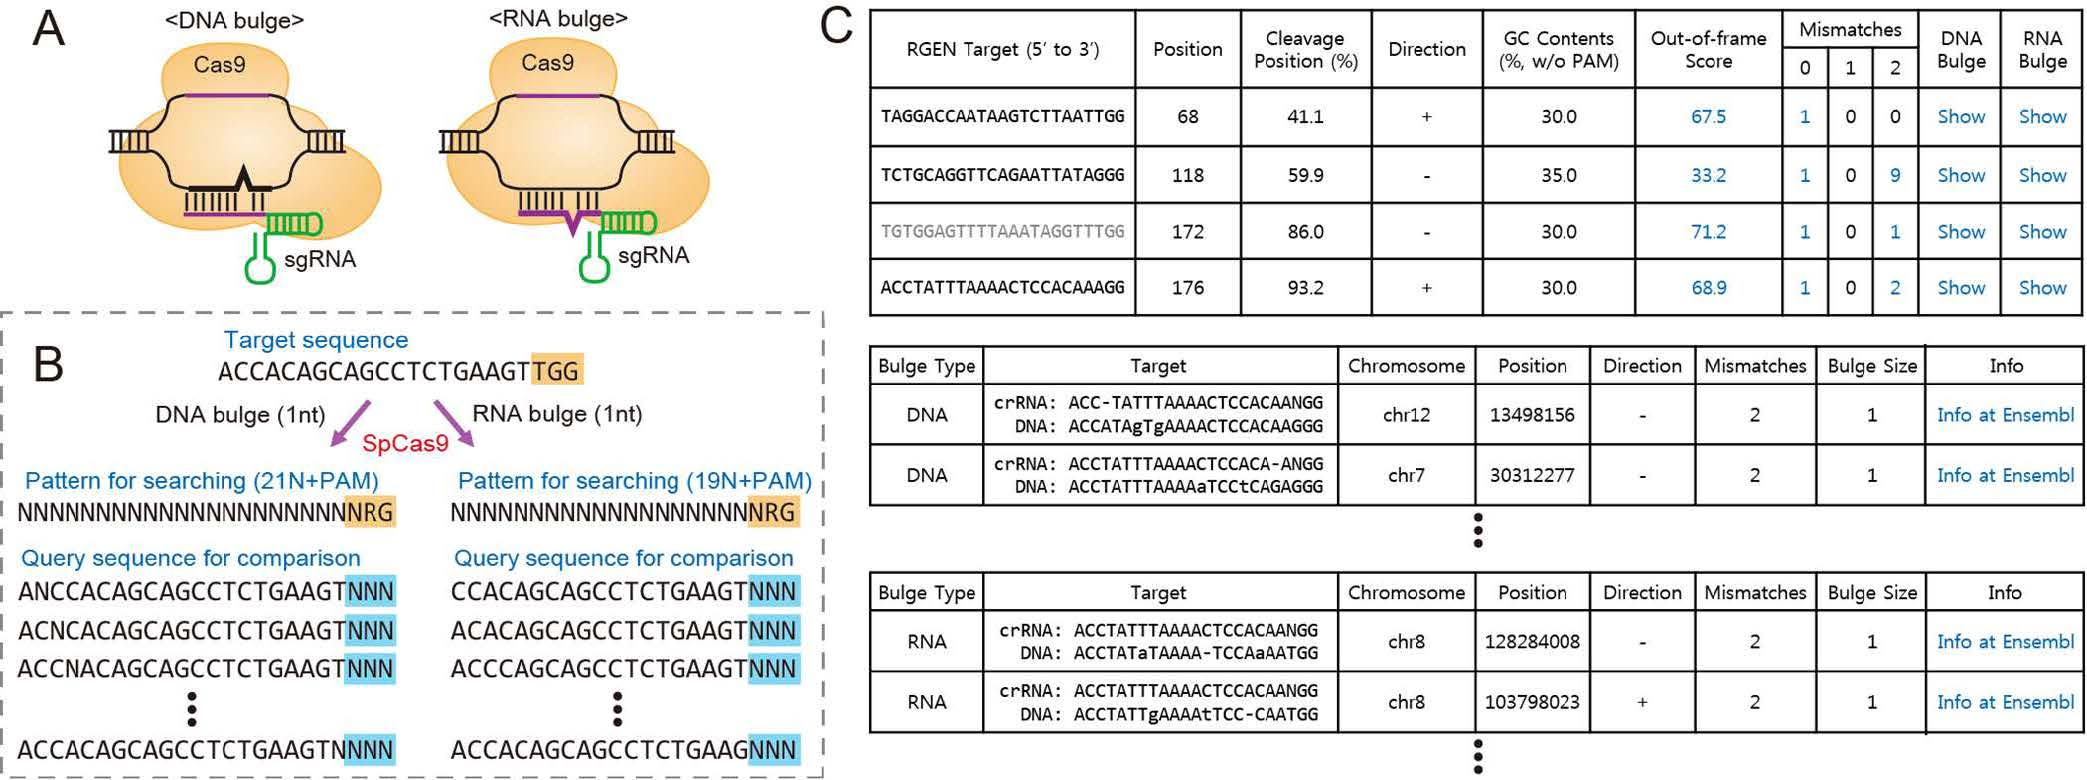
\includegraphics[width=16cm, ]{pictures/Cas-Designer.jpg}
\caption{
(الف) شماتیک مکان‌های off-tagets را با برآمدگی DNA یا RNA نشان می‌دهد. (ب) استراتژی برای  برآمدگی \lr{1-nt DNA} یا RNA بر اساس Cas-OFFinder. ج) یک مثال
از یک جدول خروجی Cas-Designer تمام gRNA های ممکن را از توالی های ورودی به همراه اطلاعات مفید (بالا) نشان می دهد. اگر کاربر روی رنگ آبی کلیک کند
عدد، کلمه یا عبارت، اطلاعات دقیق تری مانند اهداف برآمدگی DNA (وسط) یا RNA (پایین) ارائه می شود. علاوه بر این، کاربر می تواند موارد مربوطه را به دست آورد
اطلاعات ژنومی از طریق مرورگر ژنوم Ensembl \lr{Flicek)} و همکاران، 2011)، با کلیک بر روی دکمه "اطلاعات در \lr{"Ensembl}
}\label{fig:4}
\end{figure}

ابتدا Cas-Designer سایت های طرح‌های احتمالی را با یک کاربر تعریف شده [\lr{50-NGG-30} یا \lr{50-NRG-30} برای \lr{SpCas9}, \lr{50-NNAGAAW-30} برای \lr{StCas9 (Cong et al., 2013)}, \lr{50-NNNNGMTT-30} برای \lr{NmCas9 (Hou et al., 2013)} و \lr{50-NNGRRT-30} برای \lr{SaCas9 (Ran et al., 2015)}] در یک توالی DNA معین  پیدا می کند. دوم، Cas-Designer
امتیاز خارج از قاب مرتبط با میکروهومولوژی را به سرعت محاسبه می کندکه با فراوانی جهش های تغییر قاب همبستگی مثبت دارد \lr{(Bae et al., 2014b)}. محتوای GC و امتیازات خارج از کادر در این مرحله موقعیت های برش را نشان می دهد.

\lr{Cas-OFFinder}
 از دو هسته OpenCL مختلف تشکیل شده است
هسته جست‌وجوگر و یک هسته مقایسه‌گر) و C++. ابتدا Cas-OFFinder فایل های داده توالی ژنوم را به صورت تک یا چندتایی در فرمت FASTA می‌خواند. سپس در هسته جستجو بارگذاری می شود که تمام سایت هایی را که شامل یک توالی PAM در کل ژنوم هستند، کامپایل می کند. برای جستجو و انتخاب سریع و مؤثر این سایت‌های خاص، هسته جستجوگر به‌طور مستقل روی هر واحد محاسباتی یک پردازنده اجرا می‌شود، یعنی همه فرآیندهای جستجو در واحدهای محاسباتی به طور همزمان انجام می‌شوند.


\subsection{E-CRISP ~\cite{E-CRISP}}
\begin{wrapfigure}{l}{8.5cm}
\centering
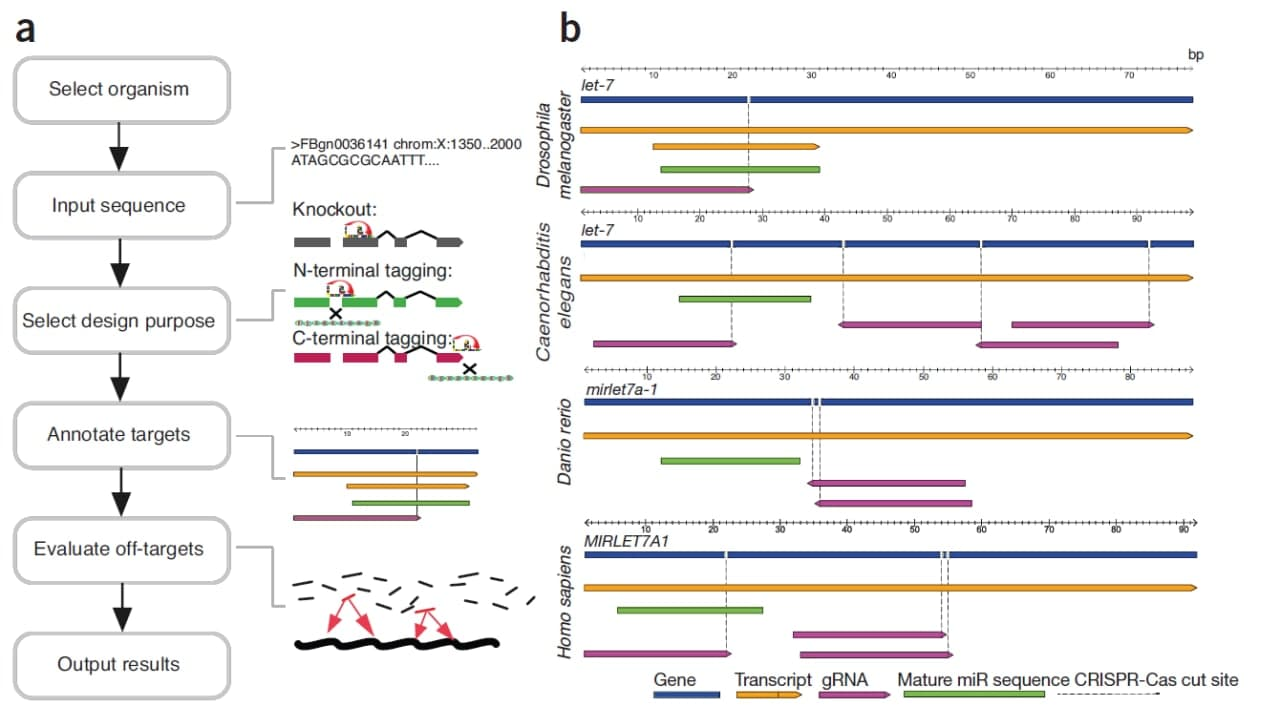
\includegraphics[width=10cm, ]{pictures/ecrispr.jpg}
\caption{
الگوریتم E-CRISP
}\label{wrap-fig:4}
\end{wrapfigure}

در اینجا ما E-CRISP، یک برنامه وب برای طراحی توالی های gRNA را توصیف می کنیم. (الف) مراحل E-CRISP. ابتدا کاربر ارگانیسم و دنباله هدف را انتخاب می کند. این هدف می تواند یک نماد ژن، یک شناسه ENSEMBL یا یک توالی FASTA باشد. دوم، کاربر هدف آزمایش ویرایش را مشخص می کند. بسته به هدف، E-CRISP مناطق مختلفی از توالی ژن را مورد هدف قرار می دهد.
سوم، E-CRISP نتایج را با توجه به اطلاعات حاشیه نویسی ژن فیلتر می کند. چهارم، اهداف خارج از هدف بر اساس تراز توالی هر طرح با ژنوم مرجع تجزیه و تحلیل می شوند. در نهایت، E-CRISP یک صفحه خروجی تعریف شده توسط کاربر تولید می کند.
(ب) RNA های راهنما در برابر جایگاه let-7 گونه های مشخص شده طراحی شده اند. توالی و محل gRNA های بالغ از miRBase بازیابی شده است. این خروجی انعطاف‌پذیر و پارامترهای طراحی آزمایش‌گرا را فراهم می‌کند، طراحی کتابخانه‌های متعدد و در نتیجه تجزیه و تحلیل سیستماتیک تأثیر پارامترهای مختلف را ممکن می‌سازد. E-CRISP توالی‌های هدف مکمل gRNA را شناسایی می‌کند که به یک موتیف که از سمت  '۳ مجاور به A)G یا N(G ختم می‌شود، که برای هسته Cas9 مورد نیاز است تا رشته دوگانه DNA را برش دهد. E-CRISP از یک رویکرد نمایه سازی سریع برای یافتن مکان های اتصال و یک درخت فاصله دودویی برای حاشیه نویسی سریع سایت های هدف gRNA احتمالی استفاده می کند. با استفاده از این الگوریتم‌ها، می‌توان در چند ساعت کتابخانه‌هایی در مقیاس ژنومی برای چندین موجود زنده ایجاد کرد.
\subsection{CRISPOR~\cite{CRISPOR}}
\begin{wrapfigure}{l}{8cm}
\centering
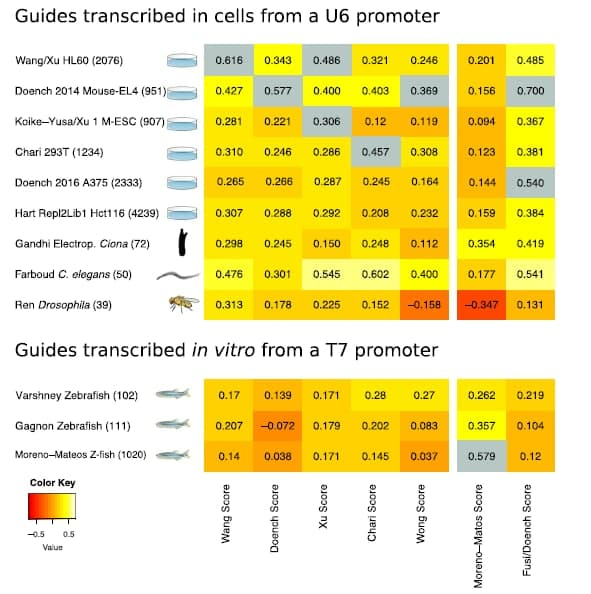
\includegraphics[width=9.5cm, ]{pictures/CRISPOR.jpg}
\caption{
هم بستگی اسپیرمن بین امتیاز موثر بودن و داده‌ها	
}\label{wrap-fig:4}
\end{wrapfigure}
CRISPOR
 وب‌سایتی است که به انتخاب و بیان توالی‌های راهنمای CRISPR کمک می‌کند، که در دو مقاله توضیح داده شده است (Gen Biol 2016 و NAR 2018). در حالت پیش فرض، کاربر یک توالی DNA ورودی را چسبانده و ژنوم را انتخاب می کند. سپس CRISPOR راهنماها را در توالی ورودی فهرست می‌کند و اطلاعات مربوط به آنها را که در پایگاه‌های اطلاعاتی و الگوریتم‌ها یافت می‌شود، از جمله انواع ژنوم، امتیازهای پیش‌بینی‌شده off-targets و هدف، اضافه می‌کند. برای هر دنباله راهنما، پرایمرهای مختلفی طراحی شده است، به عنوان مثال. برای تقویت هدف، RNA های راهنما را با رونویسی آزمایشگاهی پس از بازپخت پرایمرهای همپوشانی یا برای شبیه سازی در پلاسمیدهای AddGene تولید کنید.
برای پیش‌بینی، داده‌ها را از هشت مطالعه \lr{،off-target} SpCas9 جمع‌آوری کرده و آنها را با سایت‌های پیش‌بینی‌شده توسط الگوریتم‌های محبوب مقایسه کردند و دریافتند که پیش‌بینی‌های off-target مبتنی بر توالی بسیار قابل اعتماد هستند، و اکثر اهداف خارج از هدف را با نرخ جهش بالاتر از 0.1٪ شناسایی می‌کنند، در حالی که تعداد موارد مثبت کاذب را می‌توان تا حد زیادی با یک برش روی این امتیاز حساسیت را افزایش داد. با توجه به آزمایشات مقاله به این درس یافتند که امتیاز موثر بودن به شدت به این بستگی دارد که آیا RNA راهنما از یک پروموتر U6 بیان می‌شود یا در شرایط آزمایشگاهی رونویسی می‌شود و با این ویژگی نشان دادند که میتوان با زمان مناسب پیش‌بینی مناسبی ارائه داد.
\section{روش‌های یادگیری ژرف}
\subsection{پیش‌بینی off-target به کمک یادگیری ژرف}
\begin{wrapfigure}{l}{8cm}
\centering
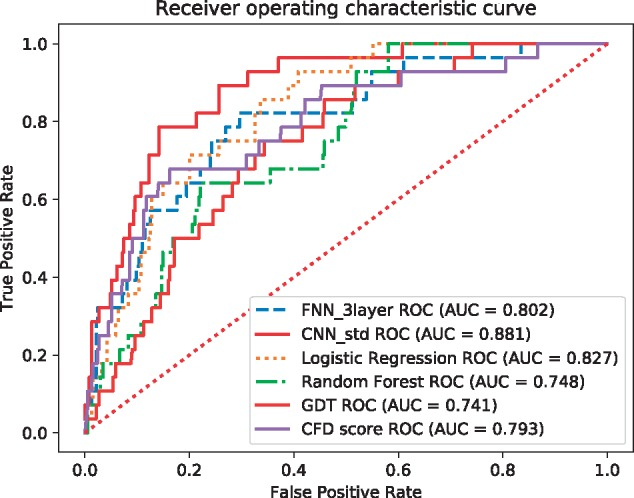
\includegraphics[width=9cm, ]{pictures/DeepLearning.jpg}
\caption{
هم بستگی اسپیرمن بین امتیاز موثر بودن و داده‌ها ~\cite{chart}
}\label{wrap-fig:4}
\end{wrapfigure}
پیش‌بینی جهش‌های خارج از هدف در CRISPR-Cas9 به دلیل ارتباط آن با تحقیقات ویرایش ژن یک موضوع پرپژوهشی است. روش های پیش بینی مختلفی توسعه یافته‌اند. با این حال، اکثر آنها فقط امتیازات را بر اساس عدم تطابق با دنباله راهنما در CRISPR-Cas9 محاسبه کردند. بنابراین، روش‌های پیش‌بینی موجود قادر به مقیاس‌بندی و بهبود عملکرد خود با گسترش سریع داده‌های تجربی در CRISPR-Cas9 نیستند. علاوه بر این، روش‌های موجود هنوز نمی‌توانند دقت کافی را در پیش‌بینی‌های خارج از هدف برای ویرایش ژن در سطح بالینی برآورده کنند. برای رفع این مشکل، مقاله دو الگوریتم را با استفاده از شبکه‌های عصبی عمیق برای پیش‌بینی جهش‌های off-target در ویرایش ژن CRISPR-Cas9 طراحی و پیاده‌سازی می‌کنیم (به توجه به اطلاعات اولین الگوریتم ماشینی). این مدل‌ها بر روی مجموعه داده‌های اخیراً منتشر شده، مجموعه داده‌های CRISPOR، برای معیار عملکرد، آموزش دیده و آزمایش شدند. یکی دیگر از مجموعه داده شناسایی شده توسط GUIDE-seq برای ارزیابی بیشتر مورد استفاده قرار گرفت. مقاله نشان می‌دهد که شبکه عصبی کانولوشن بهترین عملکرد را در مجموعه داده‌های CRISPOR به دست می‌آورد، و سطح طبقه‌بندی متوسط ​​زیر منحنی ۹۷.۰ درصد را تحت اعتبارسنجی متقاطع 5 برابری طبقه‌بندی شده به دست می‌آورد. جالب اینجاست که شبکه عصبی پیشخور عمیق نیز می‌تواند با میانگین ۹۷.۰ در همان تنظیمات رقابتی باشد. ما دو مدل شبکه عصبی عمیق را با روش‌های پیشرفته پیش‌بینی off-target (مانند CFD، MIT، CROP-IT، و CCTop) و سه مدل سنتی یادگیری ماشین (یعنی جنگل تصادفی، درخت‌های تقویت‌کننده گرادیان، و رگرسیون لجستیک) در هر دو مجموعه داده از نظر مقادیر AUC، نشان دهنده لبه های رقابتی الگوریتم های پیشنهادی است. تحلیل های اضافی برای بررسی دلایل زمینه ای از دیدگاه های مختلف انجام می شود.

\subsection{CCTop~\cite{CCTop}}
این روش برای اینکه طرح‌های مختلف که به صورت N20NGG هستند را دسته بندی کند، ابتدا با آزمایش‌های عملی طرح‌ها را به دو کلاس موٍثر و ناموثر دسته‌بندی کرد. آزمایش به این گونه بود که در محیط آزمایشگاهی طرح را به ژن طزیق می کردند و ادامه آن پیشترف هر طرح را با شمردن هدف‌های تغییر کرده در طول زمان را یاد داشت کرده. این روش بر این باور بود که ribosomal و non-ribosmal بودن ژن در تاثیر طرح موثر است پس دیتاست خود را به دو قسمت تقسیم کرده و برای طرح هر کدام sgrna موثر و ناموثر را تایین کرده. این طرخ جایگاه هر نیکلوتاید را در sgrnaهای موثر و ناموثر برسی کرده و به نتایج زیر رسیده است.\\
نحوی انتخاب موثر یا ناموثر بودن یک طرح با کمک مدل حسب مدل  Elastic-Net است که در آن اگر
 $X_i$
encode شده طرح ها باشند
و Yها امتیاز آن‌ها باشد داریم:
\\
پس از تمرین این مدل به ۲۸ ویژگی رسید که بیشتر ویژگی ها در ناحیه اسپیسر واقع شده اند و بعضی از آنها قبلا پیدا شده بود و بعضی جدید بود:
\begin{itemize}
\item Gها به شدت در موقعیت های -1 و -2 به PAM در CAS9 ترجیح داده می شوند
\item Tها در چهار موقعیت نزدیک به PAM نامطلوب هستند
\item
  نوکلئوتیدهای از '۵ به '۳، در حالی که توالی در سمت برعکس تاثیر قابل توجهی ندارد.
\item Cها در موقعیت -3 در CAS9 ترجیح داده می شوند
\item Aها در موقعیت -5 تا -12 ترجیح داده می شود.
\item G ها در موقعیت های -14 تا -17 ترجیح داده می شوند.
\end{itemize}

\section{DeepCRISPR~\cite{DeepCRISPR}}
DeepCRISPR، 
یک پلت فرم محاسباتی جامع برای یکپارچه سازی پیش‌بینی سایت sgRNA روی هدف و خارج از هدف در یک چارچوب با یادگیری عمیق، پیشی گرفتن از پیشرفته ترین ابزارهای موجود در سیلیکون. DeepCrispr [37] علاوه بر ویژگی های توالی DNA، چهار ویژگی اپی ژنتیکی را معرفی کرد و به طور خودکار اطلاعات معتبر را با استفاده از اصل Auto-encoder استخراج می کند. چندین مدل از جمله برش هدف sgRNA و پیش‌بینی تمایل خارج از هدف ایجاد شد. این پژوهشگران بر این باور بودند که خود دنباله sgrna می‌تواند اطلاعات مفید درباره موثر بودن یک توالی sgRNA بدهد به همین امر مدل خود را به دو گونه آموزش دادن با استفاده از اطلاعات اپی ژنتیکی و با اطلاعات اپی ژنتیکی که نشان میدهد که اطلاعات اپی ژنتیکی بی تاثیر نیست. 
\begin{figure}[H]
\centering
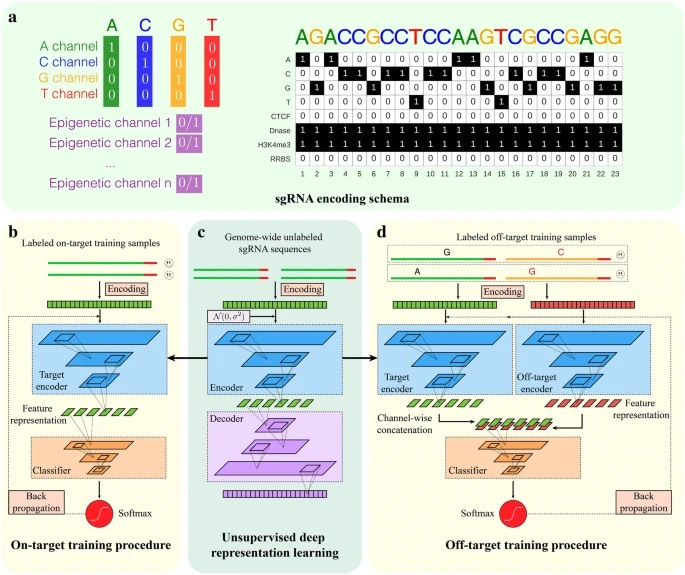
\includegraphics[width=10cm, ]{pictures/DeepCRISPR.jpg}
\caption{
DeepCRISPR
}\label{wrap-fig:4}
\end{figure}


\chapter{Methods}
\section{ensemble}
در آمار و یادگیری ماشین، روش‌های ensemble از الگوریتم‌های یادگیری چندگانه استفاده می‌کنند تا عملکرد پیش‌بینی‌کننده بهتری نسبت به هر یک از الگوریتم‌های یادگیری سازنده به‌تنهایی به‌دست آورند. ~\cite{Opitz, Polikar, Rokach} بر خلاف ensemble آماری، که معمولاً از بی نهایت مکانیک آماری استفاده میکند، یک مجموعه یادگیری ماشینی تنها از مجموعه محدود مشخصی از مدل‌های تشکیل شده است، اما معمولاً ساختار بسیار انعطاف‌پذیرتری را در بین آن گزینه‌ها امکان می‌دهد.
\subsection{تعریف}
الگوریتم های یادگیری نظارت شده وظیفه جستجو در فضای فرضیه را برای یافتن یک فرضیه مناسب انجام می دهند که پیش بینی های خوبی را با یک مسئله خاص انجام دهد.~\cite{Blockeel}

ارزیابی پیش‌بینی یک مجموعه معمولاً به محاسبات بیشتری نسبت به ارزیابی پیش‌بینی یک مدل نیاز دارد. از یک جهت، یادگیری گروهی ممکن است به عنوان راهی برای جبران الگوریتم های یادگیری ضعیف با انجام محاسبات زیاد در نظر گرفته شود. از سوی دیگر، جایگزین این است که یادگیری بسیار بیشتری را در یک سیستم غیر گروهی انجام دهید. یک سیستم ensemble ممکن است در بهبود دقت کلی برای افزایش یکسان در منابع محاسباتی، ذخیره‌سازی یا ارتباطی با استفاده از این افزایش در دو یا چند روش، کارآمدتر از افزایش استفاده از منابع برای یک روش واحد باشد. الگوریتم‌های سریع مانند درخت‌های تصمیم معمولاً در روش‌های ensemble (مثلاً جنگل‌های تصادفی) استفاده می‌شوند، اگرچه الگوریتم‌های کندتر می‌توانند از تکنیک‌های مجموعه نیز بهره ببرند.

برای اینکه بتوان از این روش‌ استفاده کرد نیاز است که ابتدا جواب این مدل‌ها یا اکسپرت‌ها را روی یک دیتای مشابه داشته باشیم، مقاله‌ی DeepCRISPR دقیقا داده ۴۲۵ دنباله sgRNA از امتیاز دهنده‌های ۵ مقاله و امتیاز مقاله خود تهیه کرده که از آنها استفاده کردیم. چندین روش ensemble برای جمع این امتیاز‌ها و رتبه بندی‌ها استفاده کردیم، مانند وزن دهی بر حسب دقت هر مدل روی یک دیتا ثابت و همین طور روش‌ LPA یا \lr{Latent Profie Analysis} که به ما مدلی برحسب پیشبینی مدل‌هایی دیگر می دهند. از این روش‌ها ما دو مدل بدست آوردیم ولی دقت این مدل‌ها همگی از مدل DeepCRISPR پایین تر بودند با آنالیز بیشتر به این نتیجه رسیدیم که این مدل‌ها بر سر بعضی نقاط شدیدا اختلاف نظر دارند که باعث تاثیر منفی در نتیجه ensemble این مدل‌ها می‌شود و با این گونه وزن دهی نمی‌توان به نتیجه بهتری رسید.

در مرحله بعدی با جنگل‌های تصادفی سعی کردیم کردیم فضای مسئله را تقسیم کنیم و بر اساس آن از امتیاز مدل‌های دیگر استفاده کنیم تا بتوانیم جواب بهتری بدست آوریم، پس از تنظیم کردن ابرپارامترها به توانستیم به مدلی بهتر از مدل‌های قبلی برسیم ولی با انجام cross-validation به این نتیجه رسیدیم که دیتای استفاده شده برای آموزش تاثیر زیادی روی دقت پیشبینی دارد و لزوما این روش همیشه از روش Deepcrispr بهتر نیست، برای بدست آوردن مدل قوی نیاز به دیتای بیشتر داشتیم.

در مرحله‌ی آخر، با توجه به اینکه اکسپرت‌ها اختلاف نظر داشتند و ensemble کردن این اکسپرت‌ها اختلاف نظر آنها را کم می کرد،‌ چهار الگوریتم، 
\lr{RandomForestRegressor ،LinearRegression ،GradientBoostingRegressor ،ExtraTreeRegressor}
را برای ensemble اکسپرت‌ها انتخاب کردیم. هر کدام از الگوریتم‌ها به تنهایی به داده آموزش حساس بودند و با انجام cross-validation لزوما به نتیجه بهتری نمی رسیدند ولی برخلاف اکسپرت‌‌های اولیه اختلاف نظر این رگرسورها خیلی کم بود و پس این متد‌ها را با هم ادغام و به نتیجه‌ی مطلوب رسیدیم، یعنی مدلی به دیتا حساس نبود و با هر فولدی باز‌ هم از روش DeepCRISPR بهتر عمل می‌کرد. 

برای اینکه مشکل داده کم را حل کنیم، ما ابتدا ۲۷۰۵ توالی مختلف را در الگوریتم‌های Cas-OFFinder، CCTop، E-Crisp، CRISPOR و Chopchop جمع آوری کردیم، که منجر بدست آمدن ۵۰هزار sgRNA یکتا شد و از آنجا که خروجی الگوریتم‌ها می توانست NaN هم باشد، با حذف این داده‌ها به ۳۶هزار sgRNA یکتا و نظر اکسپرت‌ها راجع به آن رسیدیم. تنها کافی بود که بتوانیم یک golden standard برای این داده‌ها پیدا کنیم، که متاستفانه قادر به این کار نشدیم.

\section{Attention}
موفقیت ما در روش ensemble، بر خلاف الگوریتم‌های دیگر که با استفاده از اطلاعات جانبی دیگر در مورد sgRNA بود، بر حسب نمایش دادن sgRNA در یک بردار معنا دار بود. به همین جهت ما سعی کردیم که یک بردار معنا دار از هر ‌sgRNA بسازیم و برای این امر از روش توجه استفاده کردیم.

در شبکه‌های عصبی، توجه تکنیکی است که توجه شناختی را تقلید می کند. این اثر باعث می‌شود که اثر برخی از بخش‌های ورودی افزایش یابد در حالی که بخش‌های دیگر را کاهش می‌دهد - فکر این است که شبکه باید تمرکز بیشتری را به آن بخش کوچک اما مهم داده اختصاص دهد. یادگیری اینکه کدام بخش از داده ها مهم تر از سایرین است بستگی به زمینه دارد و با نزول گرادیان آموزش داده می شود.

مکانیسم‌های مانند توجه در دهه 1990 با نام هایی مانند ماژول های ضربی، واحدهای سیگما پی و ابرشبکه ها معرفی شدند. ~\cite{Yann} انعطاف پذیری آن ناشی از نقش آن به عنوان "وزن نرم" است که می تواند در طول زمان اجرا تغییر کند، برخلاف وزنه های استاندارد که باید در زمان اجرا ثابت بمانند. کاربردهای توجه شامل حافظه در ماشین‌های تورینگ عصبی، وظایف استدلال در رایانه‌های عصبی متمایز ~\cite{Hybrid}، پردازش زبان در ترانسفورماتورها، و پردازش داده‌های چندحسی (صدا، تصاویر، ویدئو، متن) در درک‌کننده‌ها است.~\cite{nature,Vaswani, Ramachandran, Jaegle, Ray} 	

این مدل‌ها از دو قسمت نظارت شده و  نظارت نشده تشکیل شده که اولین آموزش برای پیدا کردن ساختار کلی است و دومین آموزش برای تنظیم مناسب برای امر خاص است.

در اینجا ما چند مدل مختلف مانند bert و roberta و DNAbert برای کلاس بندی sgRNAها استفاده کردیم که نتایج این مدل‌ها خیلی ضعیف بود. با توجه به آنالیزهای انجام شده به این نتیجه رسیدیم که مشکل از دیتاهای بدون لیب و با لیب استفاده شده در طول آموزش‌ها بود. برای ساخت token ابتدا از روش مرسوم kmer در DNA استفاده کردیم [7] که به این صورت است که برای هر حرف از توالی k حرف بعد از آن تکرار می‌شود. سپس این کلمات kتایی را به عنوان دیکشنری کلمات در نظر می گیریم. برای قسمت pretrain از sgRNA که خودمان ذخیره کرده بودیم و داده‌های دیگر استفاده کردیم و سپس برای تنظیمات نهایی از داده‌های مقاله DNAbert استفاده کردیم ولی نتایج آن نتایج جالبی نبود.
\chapter{Results}
\subsection{Ensemble}
نمونه‌ای از نتایج استفاده مستقیم روش‌های LPA و رگرسیون برای پیدا کردن وزن خوب بین اکسپرت‌ها
\begin{figure}[H]
\centering
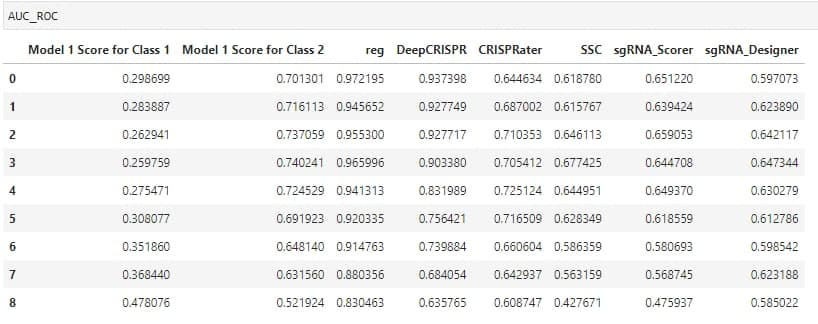
\includegraphics[width=15cm, ]{pictures/DeepCRISPR_AUR.jpg}
\caption{
AUC ROC
}\label{wrap-fig:4}
\end{figure}

\begin{figure}[H]
\centering
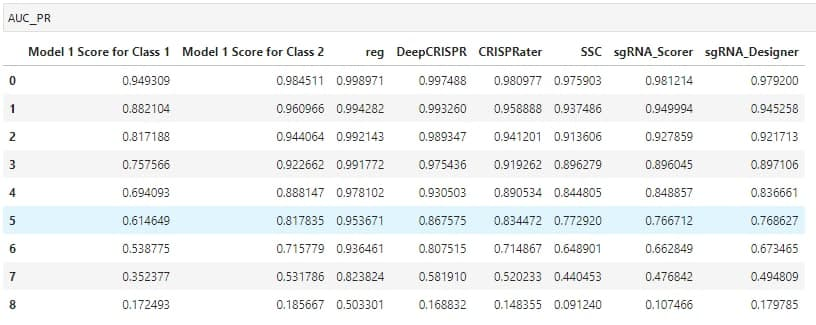
\includegraphics[width=15cm, ]{pictures/DeepCRISPR_PR.jpg}
\caption{
AUC PR
}\label{wrap-fig:4}
\end{figure}

\begin{figure}[H]
\centering
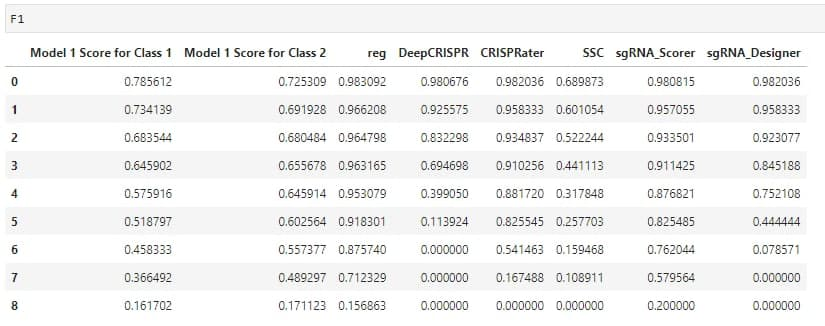
\includegraphics[width=15cm, ]{pictures/DeepCRISPR_F1.jpg}
\caption{
F1 score
}\label{wrap-fig:4}
\end{figure}

نمونه‌ای از داده‌های مقاله DeepCRISPR و امتیاز اسپیرمن بین جواب DeepCRISPR و رگرسیون درخت تصادفی
\begin{figure}[H]
\centering
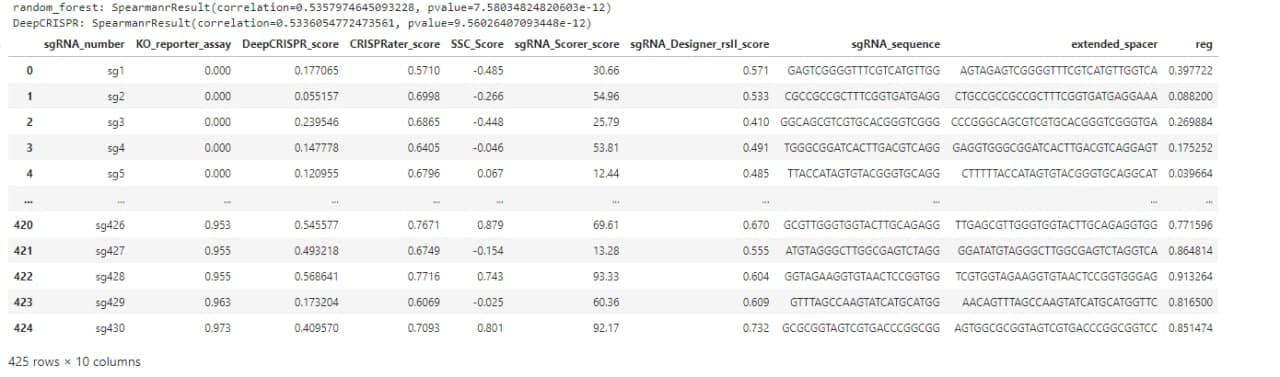
\includegraphics[width=16cm, ]{pictures/DeepCRISPR_Data.jpg}
\caption{
هم بستگی اسپیرمن بین امتیاز موثر بودن و داده‌ها
}\label{wrap-fig:4}
\end{figure}
 نمونه از امتیاز ادغام روش‌های ادغام و داده‌های که برای تست این الگوریتم استفاده شدند.
\begin{figure}[H]
\centering
\includegraphics[width=16cm, ]{pictures/best_ensemble1.jpg}
\caption{
نتیجه آموزش ل
}\label{wrap-fig:4}
\end{figure}
\begin{figure}[H]
\centering
\includegraphics[width=16cm, ]{pictures/best_ensemble2.jpg}
\caption{
هم بستگی اسپیرمن بین امتیاز موثر بودن و داده‌ها
}\label{wrap-fig:4}
\end{figure}

\subsection{Attention}
نتیجه‌ی دسته بندی بعد از آموزش به کمک مدل‌های توجه
\begin{figure}[H]
\centering
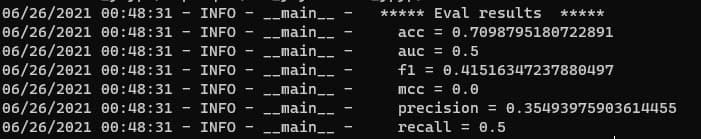
\includegraphics[width=15cm, ]{pictures/3mer.jpg}
\caption{
نتیجه تمرین به کمک 3mer، به کمک مدل DNAbert
}\label{wrap-fig:4}
\end{figure}

\begin{figure}[H]
\centering
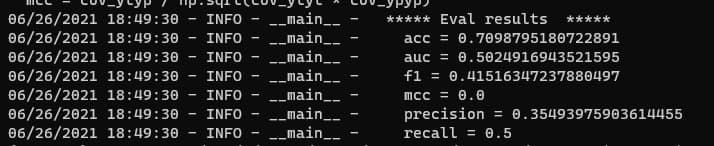
\includegraphics[width=15cm, ]{pictures/4mer.jpg}
\caption{
نتیجه تمرین به کمک 4mer، به کمک مدل DNAbert
}\label{wrap-fig:4}
\end{figure}

\begin{figure}[H]
\centering
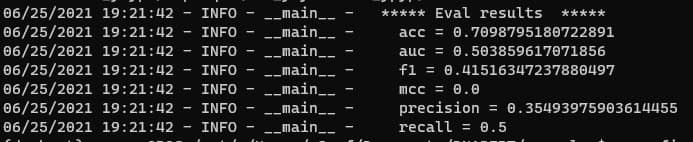
\includegraphics[width=15cm, ]{pictures/6mer.jpg}
\caption{
نتیجه تمرین به کمک 6mer، به کمک مدل DNAbert
}\label{wrap-fig:4}
\end{figure}
نتیجه آموزش مدل توجه
\begin{figure}[H]
\centering
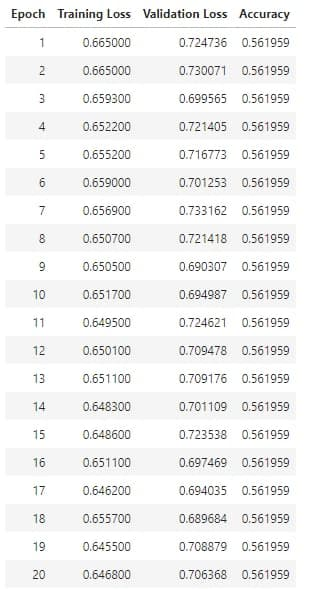
\includegraphics[width=7cm, ]{pictures/crisprBert.jpg}
\caption{
نتیجه تمرین به کمک 6mer، به کمک مدل RoBerta
}\label{wrap-fig:4}
\end{figure}

\chapter{Discussion}
دو مشکل اساسی که در داده‌ها پیدا می‌شود نویز ذاتی داده‌ها به خاطر حضور یک sgRNA در cell-lineها و ارگانیزم‌ها مختلف و نامتعادل بودن داده‌ها است چون معمولا کارشناسانی که sgRNA های مختلف را تست می‌کنند معمولا یک حس و biosی از قبل روی این sgRNAها و موفق بودن آنها دارند و یا به عبارتی دیگر به خاطر وقت و هزینه‌ی این آزمایش‌ها هیچ وقت sgRNAای که فکر میکنند اصلا خوب نیست را آزمایش نمی‌کنند که باعث به وجود آمدن دیتاست‌های نامتعادل می‌شود، فکر کردن راجع به راهی برای حذف این نویز‌ها و bios‌ها در مدل باعث می‌شود که روشی جامع برای پیش‌بینی این تاثیرگذاری sgRNAها بدست آید. 


\begin{thebibliography}{1}
\begin{latin}
\bibitem{*}{\itshape ParsiLaTeX}. \newblock {http://parsilatex.com}
\bibitem{breeding}{Selective Breeding}: \href{https://en.wikipedia.org/wiki/Plant_breeding}{\url{https://en.wikipedia.org/wiki/Plant_breeding}}
\bibitem{TED}{TED Talk}: \href{https://www.ted.com/talks/jennifer_doudna_we_can_now_edit_our_dna_but_let_s_do_it_wisely/transcript?language=fa}{\url{https://www.ted.com/talks/jennifer_doudna_we_can_now_edit_our_dna_but_let_s_do_it_wisely/transcript?language=fa}}
\bibitem{Ishino}{} { Ishino Y, Shinagawa H, Makino K, Amemura M, Nakata A. Nucleotide sequence of the iap gene, responsible for alkaline phosphatase isozyme conversion in Escherichia coli, and identification of the gene product. Journal of Bacteriology. 1987; 169, 5429–5433.}
\bibitem{Mojica}{}{Mojica, F.J. , Juez, G. \& Rodriguez-Valera, F. (1993) Transcription at different salinities of Haloferax mediterranei sequences adjacent to partially modified PstI sites. Molecular Microbiology, 9, 613–621.}
\bibitem{Patrick}{} {Patrick D. Hsu, Eric S. Lander, and Feng Zhang. Development and Applications of CRISPR-Cas9 for Genome Engineering Patrick. 2014, Cell 157(6): 1262-1278.
 4.1.3 add gene}
\bibitem{Opitz}{} {Opitz, D.; Maclin, R. (1999). "Popular ensemble methods: An empirical study". Journal of Artificial Intelligence Research. 11: 169–198. doi:10.1613/jair.614.}
\bibitem{Polikar}{} {Polikar, R. (2006). "Ensemble based systems in decision making". IEEE Circuits and Systems Magazine. 6 (3): 21–45. doi:10.1109/MCAS.2006.1688199. S2CID 18032543.}
\bibitem{Rokach}{}:{Rokach, L. (2010). "Ensemble-based classifiers". Artificial Intelligence Review. 33 (1–2): 1–39. doi:10.1007/s10462-009-9124-7. S2CID 11149239}
\bibitem{Blockeel}{} {Blockeel H. (2011). "Hypothesis Space". Encyclopedia of Machine Learning: 511–513. doi:10.1007/978-0-387-30164-8 373. ISBN 978-0-387-30768-8.}
\bibitem{Yann}{} {Yann Lecun (2020). Deep Learning course at NYU, Spring 2020, video lecture Week 6. Event occurs at 53:00. Retrieved 2021-12-13.}
\bibitem{Hybrid}{} {"Hybrid computing using a neural network with dynamic external memory". Nature. 538 (7626): 471–476. 2016-10-12. Bibcode:2016Natur.538..471G. doi:10.1038/nature20101. ISSN 1476-4687. PMID 27732574. S2CID 205251479.}
\bibitem{nature}{} {nature20101. ISSN 1476-4687. PMID 27732574. S2CID 205251479.}
\bibitem{Vaswani}{} { Vaswani, Ashish; Shazeer, Noam; Parmar, Niki; Uszkoreit, Jakob; Jones, Llion; Gomez, Aidan N.; Kaiser, Lukasz; Polosukhin, Illia (2017-12-05). "Attention Is All You Need". arXiv:1706.03762 [cs.CL].}
\bibitem{Ramachandran}{} {Ramachandran, Prajit; Parmar, Niki; Vaswani, Ashish; Bello, Irwan; Levskaya, Anselm; Shlens, Jonathon (2019-06-13). "Stand-Alone Self-Attention in Vision Models". arXiv:1906.05909 [cs.CV].}
\bibitem{Jaegle}{} {Jaegle, Andrew; Gimeno, Felix; Brock, Andrew; Zisserman, Andrew; Vinyals, Oriol; Carreira, Joao (2021-06-22). "Perceiver: General Perception with Iterative Attention". arXiv:2103.03206 [cs.CV].}
\bibitem{Ray}{} {Ray, Tiernan. "Google's Supermodel: DeepMind Perceiver is a step on the road to an AI machine that could process anything and everything". ZDNet. Retrieved 2021-08-19.}
\bibitem{DeepCRISPR}{} {Guohui Chuai, Qi Liu et al. DeepCRISPR: optimized CRISPR guide RNA design by deep learning. 2018 (Manuscript submitted)}
\bibitem{CCTop}{} {Stemmer, M., Thumberger, T., del Sol Keyer, M., Wittbrodt, J. and Mateo, J.L. CCTop: an intuitive, flexible and reliable CRISPR/Cas9 target prediction tool. PLOS ONE (2015). doi: 10.1371/journal.pone.0124633}
\bibitem{CRISPRater}{} {Labuhn, M., Adams, F. F., Ng, M., Knoess, S., Schambach, A., Charpentier, E. M., … Heckl, D. Refined sgRNA efficacy prediction improves large- and small-scale CRISPR–Cas9 applications. Nucleic Acids Research (2017). doi: 10.1093/nar/gkx1268}
\bibitem{chart}{} {Off-target predictions in CRISPR-Cas9 gene editing using deep learning
Jiecong Lin and Ka-Chun Wong, Bioinformatics. 2018 Sep 1, doi: 10.1093/bioinformatics/bty554}
\bibitem{DeepCRISPR}{} {Guohui Chuai, Qi Liu et al. DeepCRISPR: optimized CRISPR guide RNA design by deep learning. 2018 (Manuscript submitted)}
\bibitem{CRISPOR}{} {CRISPOR: intuitive guide selection for CRISPR/Cas9 genome editing experiments and screens, Jean-Paul Concordet, Maximilian Haeussler, Nucleic Acids Research, Volume 46, Issue W1, 2 July 2018, Pages W242–W245, https://doi.org/10.1093/nar/gky354}
\bibitem{E-CRISP}{} {E-CRISP: fast CRISPR target site identification , Florian Heigwer, Grainne Kerr \& Michael Boutros}
\bibitem{Cas-Designer}{} {Cas-Designer: a web-based tool for choice of CRISPR-Cas9 target sites 
Jeongbin Park, Sangsu Bae, Jin-Soo Kim, https://doi.org/10.1093/bioinformatics/btv537}
\bibitem{Cas-OFFinder}{} {Cas-OFFinder: a fast and versatile algorithm that searches for potential off-target sites of Cas9 RNA-guided endonucleases, Sangsu Bae 1, Jeongbin Park, Jin-Soo Kim, DOI: 10.1093/bioinformatics/btu048}
\bibitem{CHOPCHOP3}{} {CHOPCHOP v3: expanding the CRISPR web toolbox beyond genome editing}
\bibitem{CHOPCHOP2}{} {CHOPCHOP v2: a web tool for the next generation of CRISPR genome engineering 
Kornel Labun, Tessa G. Montague, James A. Gagnon, Summer B. Thyme, Eivind Valen}
\bibitem{CHOPCHOP}{} {CHOPCHOP: a CRISPR/Cas9 and TALEN web tool for genome editing}

\bibitem{addgene}{All you need about CRISPR:} {https://www.addgene.org/guides/crispr/}

\bibitem{Wired}{Good Overview by Wired:} {\href{https://www.wired.com/2015/07/crispr-dna-editing-2/}{\url{https://www.wired.com/2015/07/crispr-dna-editing-2/}}}
\bibitem{DNA}{DNA:} {\href{https://en.wikipedia.org/wiki/DNA}{\url{https://en.wikipedia.org/wiki/DNA}}}
\bibitem{DNA1}{} {\href{https://medlineplus.gov/genetics/understanding/basics/dna/}{\url{https://medlineplus.gov/genetics/understanding/basics/dna/}}}
\bibitem{Radiation}{Radiation research:} {\href{https://www.amusingplanet.com/2013/03/atomic-gardening-breeding-plants-with.html}{\url{https://www.amusingplanet.com/2013/03/atomic-gardening-breeding-plants-with.html}}}

\bibitem{snippets}{inserting DNA snippets into organisms:} {\href{http://www.genomenewsnetwork.org/resources/timeline/1977_Gilbert.php}{\url{http://www.genomenewsnetwork.org/resources/timeline/1977_Gilbert.php}}}

\bibitem{animal}{First genetically modified animal:} {\href{https://www.pnas.org/content/71/4/1250?tab=author-info}{\url{https://www.pnas.org/content/71/4/1250?tab=author-info}}}
\bibitem{GM}{First GM patent:} {\href{https://patents.google.com/patent/US4259444}{\url{https://patents.google.com/patent/US4259444}}}
\bibitem{GMOs}{chemicals produced by GMOs:} {\href{https://pubmed.ncbi.nlm.nih.gov/6337396/}{\url{https://pubmed.ncbi.nlm.nih.gov/6337396/}}}
\bibitem{GMOs1}{} {\href{https://pubmed.ncbi.nlm.nih.gov/15580495/}{\url{https://pubmed.ncbi.nlm.nih.gov/15580495/}}}

\bibitem{GMOs2}{} {\href{https://th.schattauer.de/contents/archive/issue/721/manuscript/9641.html}{\url{https://th.schattauer.de/contents/archive/issue/721/manuscript/9641.html}}}
\bibitem{Flavr}{Flavr Savr Tomato:}  {\href{https://calag.ucanr.edu/Archive/?article=ca.v054n04p6}{\url{https://calag.ucanr.edu/Archive/?article=ca.v054n04p6}}}
\bibitem{First}{First Human Engineering:} {\href{https://www.worldscientific.com/worldscibooks/10.1142/9542}{\url{https://www.worldscientific.com/worldscibooks/10.1142/9542}}}
\bibitem{fish}{glowing fish:} {\href{https://www.glofish.com/}{\url{https://www.glofish.com/}}}

\bibitem{CRISPR}{ CRISPR:}  {\href{http://go.nature.com/24Nhykm}{\url{http://go.nature.com/24Nhykm}}}
\bibitem{CRISPR1}{}  {\href{https://en.wikipedia.org/wiki/CRISPR}{\url{https://en.wikipedia.org/wiki/CRISPR}}}

\bibitem{HIV}{HIV cut from cells and rats with CRISPR:} {\href{https://www.nature.com/articles/531156a}{\url{https://www.nature.com/articles/531156a}}}
\bibitem{HIV1}{} {Elimination of HIV-1 Genomes from Human T-lymphoid Cells by CRISPR/Cas9 Gene Editing; Rafal Kaminski, Yilan Chen, Tracy Fischer, Ellen Tedaldi, Alessandro Napoli, Yonggang Zhang, Jonathan Karn, Wenhui Hu \& Kamel Khalili }
\bibitem{HIV2}{first human CRISPR trials fighting cancer:} {\href{https://time.com/4340722/hiv-removed-using-crispr/}{\url{https://time.com/4340722/hiv-removed-using-crispr/}}}
\bibitem{HIV3}{first human CRISPR trial approved by Chinese for August 2016} {\href{https://www.nature.com/articles/nature.2016.20137}{\url{https://www.nature.com/articles/nature.2016.20137}}}
\bibitem{Kurzgesagt – In a Nutshell}{}  {\href{https://www.youtube.com/watch?v=jAhjPd4uNFY\&t=122s}{\url{https://www.youtube.com/watch?v=jAhjPd4uNFY\&t=122s}}}




\end{latin}

\end{thebibliography}
\printindex
\begin{latin}
\begin{abstract}
Clustered Regularly Interspaced Short Palindromic Repeats, or in short, CRISPR is a relatively new
technology that enables geneticists and medical researchers to edit parts of the genome by removing,
adding, or altering parts of the DNA. Initially found in the genomes of prokaryotic organisms such as
bacteria and archaea, this technology can cure many illnesses such as blindness and cancer. A significant
issue for a practical application of CRISPR systems is accurately predicting the single guide RNA
(sgRNA) on-target efficacy and off-target sensitivity. While some methods classify these designs, most
algorithms are on separate data with different genes and cells. The lack of generalizability of these methods
hinders the use of this guide in clinical trials since, for each treatment, the process must be designed
with its unique dataset, which has its own problems. Here we are trying to solve the generalizability
of this problem and present general and targeted prediction models that will help researchers optimize
the design of sgRNAs with high sensitivity. First, we tackled the problem by leveraging Latent Profile
Analysis and attention-based models to combine previous algorithms. However, the results obtained
using these methods were not satisfactory since the data was noisy. Finally,
we proposed a novel Ensemble Learning, which is compatible in terms of accuracy. However, our
method provides the advantage of generalizability, allowing the model to offer insightful estimates to
RNA on-target efficiency that can quickly learn to predict even in new genes or cells.
\end{abstract}
\end{latin}

\university{Sharif University of Technology }
\department{Department of Mathematical Sciences}
\thesis{ M.Sc. Thesis}
\subject{‌Applied Mathematics}
\author{Mohammad Rostami}
\title{A study in genome editing with clustered regularly interspaced short palindromic repeats}
\supervisor{Dr. Mohsen Sharifi Tabar}
\secsupervisor{Dr. Hamidreza Rabiee}%در صورت نیاز
\advisor{Dr. Mohammad Hossein Rohban}%در صورت نیاز
\date{\latintoday}
\makethesisenglishtitle

\end{document}
